%%%%%%%%%%%%%%%%%%%%%%%%%%%%%%%%%%%%%%%%%%%%%%%%%%%%%%%%%%%

%%%%%%%%%%%%%%%%%%%%%%%%%%%%%%%%%%%%%%%%%%%%%%%%%%%%%%%%%%%

%% document class
\documentclass[a4paper,11pt,oneside]{book}

%% packages
%% packages

\usepackage{blindtext} % needed for creating dummy text passages
%\usepackage{ngerman} % needed for German default language
\usepackage{amsmath} % needed for command eqref
\usepackage{amssymb} % needed for math fonts
\usepackage[
	colorlinks=true
	,breaklinks
	%,ngerman
	]{hyperref} % needed for creating hyperlinks in the document, the option colorlinks=true gets rid of the awful boxes, breaklinks breaks lonkg links (list of figures), and ngerman sets everything for german as default hyperlinks language
\usepackage[hyphenbreaks]{breakurl} % ben�tigt f�r das Brechen von URLs in Literaturreferenzen, hyphenbreaks auch bei links, die �ber eine Seite gehen (mit hyphenation).
\usepackage{xcolor}
\definecolor{c1}{rgb}{0,0,1} % blue
\definecolor{c2}{rgb}{0,0.3,0.9} % light blue
\definecolor{c3}{rgb}{0.3,0,0.9} % red blue
\hypersetup{
    linkcolor={c1}, % internal links
    citecolor={c2}, % citations
    urlcolor={c3} % external links/urls
}
%\usepackage{cite} % needed for cite
\usepackage[round,authoryear]{natbib} % needed for cite and abbrvnat bibliography style
\usepackage[nottoc]{tocbibind} % needed for displaying bibliography and other in the table of contents
\usepackage{graphicx} % needed for \includegraphics 
\usepackage{longtable} % needed for long tables over pages
\usepackage{bigstrut} % needed for the command \bigstrut
\usepackage{enumerate} % needed for some options in enumerate
\usepackage{array}
\usepackage{textgreek}
\usepackage{todonotes} % needed for todos
\usepackage{makeidx} % needed for creating an index
\makeindex
\usepackage{placeins}
\usepackage [english]{babel}
\usepackage [autostyle, english = american]{csquotes}
\MakeOuterQuote{"}
\usepackage{multirow}
\usepackage{dcolumn}
\usepackage{array}
\usepackage{makecell}

%% page settings
%% page settings

\usepackage[top=2cm, bottom=1.8cm,left=2.5cm,right=2.5cm]{geometry} % needed for page border settings
\parindent=0cm % for space of first line of new text block
\sloppy % for writing with hyphenless justification (tries to)
\hyphenation{} % use hyphenation of tolerance parameters, http://www.jr-x.de/publikationen/latex/tipps/zeilenumbruch.html
\hyphenpenalty=10000
\exhyphenpenalty=10000
\usepackage{fancyhdr} % needed for head and foot options

%% own commands
%\newcommand{\tbi}[1]{\textbf{\textit{#1}}}
%% my macros

%% Text fomats
\newcommand{\tbi}[1]{\textbf{\textit{#1}}}

%% Math fonts
\newcommand{\bbA}{\mathbb{A}}
\newcommand{\bbB}{\mathbb{B}}
\newcommand{\bbC}{\mathbb{C}}
\newcommand{\bbD}{\mathbb{D}}
\newcommand{\bbE}{\mathbb{E}}
\newcommand{\bbF}{\mathbb{F}}
\newcommand{\bbG}{\mathbb{G}}
\newcommand{\bbH}{\mathbb{H}}
\newcommand{\bbI}{\mathbb{I}}
\newcommand{\bbJ}{\mathbb{J}}
\newcommand{\bbK}{\mathbb{K}}
\newcommand{\bbL}{\mathbb{L}}
\newcommand{\bbM}{\mathbb{M}}
\newcommand{\bbN}{\mathbb{N}}
\newcommand{\bbO}{\mathbb{O}}
\newcommand{\bbP}{\mathbb{P}}
\newcommand{\bbQ}{\mathbb{Q}}
\newcommand{\bbR}{\mathbb{R}}
\newcommand{\bbS}{\mathbb{S}}
\newcommand{\bbT}{\mathbb{T}}
\newcommand{\bbU}{\mathbb{U}}
\newcommand{\bbV}{\mathbb{V}}
\newcommand{\bbW}{\mathbb{W}}
\newcommand{\bbX}{\mathbb{X}}
\newcommand{\bbY}{\mathbb{Y}}
\newcommand{\bbZ}{\mathbb{Z}}
\newcommand{\imp}[1]{\underline{\textit{#1}}}

%%%%%%%%%%%%%%%%%%%%%%%%%%%%%%%%%%%%%%%%%%%%%%%%%%%%%%%%%%%

\begin{document}
	
	%%%%%%%%%%%%%%%%%%%%%%%%%%%%%%%%%%%%%%%%%%%%%%%%%%%%%%%%%%%
	%%%%%%%%%%%%%%%%%%%%%%%%%%%%%%%%%%%%%%%%%%%%%%%%%%%%%%%%%%%
	%%%%%%%%%%%%%%%%%%%%%%%%%%%%%%%%%%%%%%%%%%%%%%%%%%%%%%%%%%%
	
	%\pagestyle{empty}
	%\title{Basic elements for writing a book/thesis using \LaTeX}
	%\autr{Mauricio Lobos}
	%\date{}
	%\maketitle
	%%%%%%%%%%%%%%%%%%%%%%%%%%%%%%%%%%%%%%%%%
% University Assignment Title Page 
% LaTeX Template
% Version 1.0 (27/12/12)
%
% This template has been downloaded from:
% http://www.LaTeXTemplates.com
%
% Original author:
% WikiBooks (http://en.wikibooks.org/wiki/LaTeX/Title_Creation)
%
% License:
% CC BY-NC-SA 3.0 (http://creativecommons.org/licenses/by-nc-sa/3.0/)
% 
% Instructions for using this template:
% This title page is capable of being compiled as is. This is not useful for 
% including it in another document. To do this, you have two options: 
%
% 1) Copy/paste everything between \begin{document} and \end{document} 
% starting at \begin{} and paste this into another LaTeX file where you 
% want your title page.
% OR
% 2) Remove everything outside the \begin{titlepage} and \end{titlepage} and 
% move this file to the same directory as the LaTeX file you wish to add it to. 
% Then add %%%%%%%%%%%%%%%%%%%%%%%%%%%%%%%%%%%%%%%%%
% University Assignment Title Page 
% LaTeX Template
% Version 1.0 (27/12/12)
%
% This template has been downloaded from:
% http://www.LaTeXTemplates.com
%
% Original author:
% WikiBooks (http://en.wikibooks.org/wiki/LaTeX/Title_Creation)
%
% License:
% CC BY-NC-SA 3.0 (http://creativecommons.org/licenses/by-nc-sa/3.0/)
% 
% Instructions for using this template:
% This title page is capable of being compiled as is. This is not useful for 
% including it in another document. To do this, you have two options: 
%
% 1) Copy/paste everything between \begin{document} and \end{document} 
% starting at \begin{} and paste this into another LaTeX file where you 
% want your title page.
% OR
% 2) Remove everything outside the \begin{titlepage} and \end{titlepage} and 
% move this file to the same directory as the LaTeX file you wish to add it to. 
% Then add %%%%%%%%%%%%%%%%%%%%%%%%%%%%%%%%%%%%%%%%%
% University Assignment Title Page 
% LaTeX Template
% Version 1.0 (27/12/12)
%
% This template has been downloaded from:
% http://www.LaTeXTemplates.com
%
% Original author:
% WikiBooks (http://en.wikibooks.org/wiki/LaTeX/Title_Creation)
%
% License:
% CC BY-NC-SA 3.0 (http://creativecommons.org/licenses/by-nc-sa/3.0/)
% 
% Instructions for using this template:
% This title page is capable of being compiled as is. This is not useful for 
% including it in another document. To do this, you have two options: 
%
% 1) Copy/paste everything between \begin{document} and \end{document} 
% starting at \begin{} and paste this into another LaTeX file where you 
% want your title page.
% OR
% 2) Remove everything outside the \begin{titlepage} and \end{titlepage} and 
% move this file to the same directory as the LaTeX file you wish to add it to. 
% Then add \input{./title_page_1.tex} to your LaTeX file where you want your
% title page.
%
%%%%%%%%%%%%%%%%%%%%%%%%%%%%%%%%%%%%%%%%%

%----------------------------------------------------------------------------------------
%	PACKAGES AND OTHER DOCUMENT CONFIGURATIONS
%----------------------------------------------------------------------------------------

%\documentclass[12pt]{article}
%
%\begin{document}

\begin{titlepage}
	

\newcommand{\HRule}{\rule{\linewidth}{0.5mm}} % Defines a new command for the horizontal lines, change thickness here

\center % Center everything on the page
 
%----------------------------------------------------------------------------------------
%	HEADING SECTIONS
%----------------------------------------------------------------------------------------
\begin{minipage}[b]{0.4\textwidth}
	%\begin{flushleft} \large
	\begin{center}
		
\includegraphics[width=0.5\textwidth]{figures/download}\\[1cm] % Include a department/university logo - this will require the graphicx package
		%\end{flushleft}
	\end{center}
\end{minipage}
\vspace{1.5cm}



\textsc{\LARGE Department of Financial Mathematics}\\[1.5cm] % Name of your university/college
\textsc{\Large }\\[0.5cm] % Major heading such as course name
\textsc{\large }\\[0.5cm] % Minor heading such as course title

%----------------------------------------------------------------------------------------
%	TITLE SECTION
%----------------------------------------------------------------------------------------

\HRule \\[0.5cm]
{ \huge \bfseries Comparison of Forecasting Models for Value at Risk}\\[0.1cm] % Title of your document
\HRule \\[1.5cm]
\vspace{2.5cm}
 
%----------------------------------------------------------------------------------------
%	AUTHOR SECTION
%----------------------------------------------------------------------------------------


\begin{minipage}{0.4\textwidth}
\begin{flushleft} \large
\emph{Author:}\\
Hafees Adebayo \textsc{Yusuff} % Your name
\end{flushleft}
\end{minipage}
~
\begin{minipage}{0.4\textwidth}
\begin{flushleft} \large
\emph{Supervisor:} \\
Prof. Ralf \textsc{Korn} % Supervisor's Name
\end{flushleft}
\end{minipage}\\[4cm]

% If you don't want a supervisor, uncomment the two lines below and remove the section above
%\Large \emph{Author:}\\
%John \textsc{Smith}\\[3cm] % Your name

%----------------------------------------------------------------------------------------

%	DATE SECTION
%----------------------------------------------------------------------------------------

{\large \today}\\[3cm] % Date, change the \today to a set date if you want to be precise
\vspace{2.5cm}


A thesis submitted in fulfilment of the requirements for the degree of
Master of Science

%----------------------------------------------------------------------------------------
%	LOGO SECTION
%----------------------------------------------------------------------------------------

%~
%\begin{minipage}[b]{0.4\textwidth}
%\begin{flushleft} \large
%
\includegraphics[width=0.5\textwidth]{figures/download (1)}
%\end{flushleft}
%\end{minipage}

%----------------------------------------------------------------------------------------

\vfill % Fill the rest of the page with whitespace
\end{titlepage}



\thispagestyle{empty}

\newpage\null\thispagestyle{empty}\newpage


\begin{titlepage}
	\textbf{\LARGE Declaration of Authorship}\newline\newline
	

		
		I, Hafees Adebayo YUSUFF, hereby declare the following thesis titled "Comparison of forecasting models for value at risk" to be my own work and I confirm that:
			\begin{itemize}
		\item[$\bullet$] The thesis I am submitting is entirely my own work except where otherwise indicated.
		
		\item[$\bullet$] It has not been submitted, either partially or in full, for a qualification at this or any other University.
	
	\item[$\bullet$] I have clearly signalled the presence of all material I have quoted from other sources,
	including any diagrams, charts, tables or graphs.
	
	\item[$\bullet$] I have acknowledged appropriately any assistance I have received.
	
	\end{itemize}
	
	\vspace*{4em}\noindent
	\hfill%
	\begin{tabular}[t]{c}
		\rule{10em}{0.4pt}\\ Signature
	\end{tabular}%
	\hfill%
	\begin{tabular}[t]{c}
		\rule{10em}{0.4pt}\\ Date
	\end{tabular}%
	\hfill\strut


\end{titlepage}
 to your LaTeX file where you want your
% title page.
%
%%%%%%%%%%%%%%%%%%%%%%%%%%%%%%%%%%%%%%%%%

%----------------------------------------------------------------------------------------
%	PACKAGES AND OTHER DOCUMENT CONFIGURATIONS
%----------------------------------------------------------------------------------------

%\documentclass[12pt]{article}
%
%\begin{document}

\begin{titlepage}
	

\newcommand{\HRule}{\rule{\linewidth}{0.5mm}} % Defines a new command for the horizontal lines, change thickness here

\center % Center everything on the page
 
%----------------------------------------------------------------------------------------
%	HEADING SECTIONS
%----------------------------------------------------------------------------------------
\begin{minipage}[b]{0.4\textwidth}
	%\begin{flushleft} \large
	\begin{center}
		
\includegraphics[width=0.5\textwidth]{figures/download}\\[1cm] % Include a department/university logo - this will require the graphicx package
		%\end{flushleft}
	\end{center}
\end{minipage}
\vspace{1.5cm}



\textsc{\LARGE Department of Financial Mathematics}\\[1.5cm] % Name of your university/college
\textsc{\Large }\\[0.5cm] % Major heading such as course name
\textsc{\large }\\[0.5cm] % Minor heading such as course title

%----------------------------------------------------------------------------------------
%	TITLE SECTION
%----------------------------------------------------------------------------------------

\HRule \\[0.5cm]
{ \huge \bfseries Comparison of Forecasting Models for Value at Risk}\\[0.1cm] % Title of your document
\HRule \\[1.5cm]
\vspace{2.5cm}
 
%----------------------------------------------------------------------------------------
%	AUTHOR SECTION
%----------------------------------------------------------------------------------------


\begin{minipage}{0.4\textwidth}
\begin{flushleft} \large
\emph{Author:}\\
Hafees Adebayo \textsc{Yusuff} % Your name
\end{flushleft}
\end{minipage}
~
\begin{minipage}{0.4\textwidth}
\begin{flushleft} \large
\emph{Supervisor:} \\
Prof. Ralf \textsc{Korn} % Supervisor's Name
\end{flushleft}
\end{minipage}\\[4cm]

% If you don't want a supervisor, uncomment the two lines below and remove the section above
%\Large \emph{Author:}\\
%John \textsc{Smith}\\[3cm] % Your name

%----------------------------------------------------------------------------------------

%	DATE SECTION
%----------------------------------------------------------------------------------------

{\large \today}\\[3cm] % Date, change the \today to a set date if you want to be precise
\vspace{2.5cm}


A thesis submitted in fulfilment of the requirements for the degree of
Master of Science

%----------------------------------------------------------------------------------------
%	LOGO SECTION
%----------------------------------------------------------------------------------------

%~
%\begin{minipage}[b]{0.4\textwidth}
%\begin{flushleft} \large
%
\includegraphics[width=0.5\textwidth]{figures/download (1)}
%\end{flushleft}
%\end{minipage}

%----------------------------------------------------------------------------------------

\vfill % Fill the rest of the page with whitespace
\end{titlepage}



\thispagestyle{empty}

\newpage\null\thispagestyle{empty}\newpage


\begin{titlepage}
	\textbf{\LARGE Declaration of Authorship}\newline\newline
	

		
		I, Hafees Adebayo YUSUFF, hereby declare the following thesis titled "Comparison of forecasting models for value at risk" to be my own work and I confirm that:
			\begin{itemize}
		\item[$\bullet$] The thesis I am submitting is entirely my own work except where otherwise indicated.
		
		\item[$\bullet$] It has not been submitted, either partially or in full, for a qualification at this or any other University.
	
	\item[$\bullet$] I have clearly signalled the presence of all material I have quoted from other sources,
	including any diagrams, charts, tables or graphs.
	
	\item[$\bullet$] I have acknowledged appropriately any assistance I have received.
	
	\end{itemize}
	
	\vspace*{4em}\noindent
	\hfill%
	\begin{tabular}[t]{c}
		\rule{10em}{0.4pt}\\ Signature
	\end{tabular}%
	\hfill%
	\begin{tabular}[t]{c}
		\rule{10em}{0.4pt}\\ Date
	\end{tabular}%
	\hfill\strut


\end{titlepage}
 to your LaTeX file where you want your
% title page.
%
%%%%%%%%%%%%%%%%%%%%%%%%%%%%%%%%%%%%%%%%%

%----------------------------------------------------------------------------------------
%	PACKAGES AND OTHER DOCUMENT CONFIGURATIONS
%----------------------------------------------------------------------------------------

%\documentclass[12pt]{article}
%
%\begin{document}

\begin{titlepage}
	

\newcommand{\HRule}{\rule{\linewidth}{0.5mm}} % Defines a new command for the horizontal lines, change thickness here

\center % Center everything on the page
 
%----------------------------------------------------------------------------------------
%	HEADING SECTIONS
%----------------------------------------------------------------------------------------
\begin{minipage}[b]{0.4\textwidth}
	%\begin{flushleft} \large
	\begin{center}
		
\includegraphics[width=0.5\textwidth]{figures/download}\\[1cm] % Include a department/university logo - this will require the graphicx package
		%\end{flushleft}
	\end{center}
\end{minipage}
\vspace{1.5cm}



\textsc{\LARGE Department of Financial Mathematics}\\[1.5cm] % Name of your university/college
\textsc{\Large }\\[0.5cm] % Major heading such as course name
\textsc{\large }\\[0.5cm] % Minor heading such as course title

%----------------------------------------------------------------------------------------
%	TITLE SECTION
%----------------------------------------------------------------------------------------

\HRule \\[0.5cm]
{ \huge \bfseries Comparison of Forecasting Models for Value at Risk}\\[0.1cm] % Title of your document
\HRule \\[1.5cm]
\vspace{2.5cm}
 
%----------------------------------------------------------------------------------------
%	AUTHOR SECTION
%----------------------------------------------------------------------------------------


\begin{minipage}{0.4\textwidth}
\begin{flushleft} \large
\emph{Author:}\\
Hafees Adebayo \textsc{Yusuff} % Your name
\end{flushleft}
\end{minipage}
~
\begin{minipage}{0.4\textwidth}
\begin{flushleft} \large
\emph{Supervisor:} \\
Prof. Ralf \textsc{Korn} % Supervisor's Name
\end{flushleft}
\end{minipage}\\[4cm]

% If you don't want a supervisor, uncomment the two lines below and remove the section above
%\Large \emph{Author:}\\
%John \textsc{Smith}\\[3cm] % Your name

%----------------------------------------------------------------------------------------

%	DATE SECTION
%----------------------------------------------------------------------------------------

{\large \today}\\[3cm] % Date, change the \today to a set date if you want to be precise
\vspace{2.5cm}


A thesis submitted in fulfilment of the requirements for the degree of
Master of Science

%----------------------------------------------------------------------------------------
%	LOGO SECTION
%----------------------------------------------------------------------------------------

%~
%\begin{minipage}[b]{0.4\textwidth}
%\begin{flushleft} \large
%
\includegraphics[width=0.5\textwidth]{figures/download (1)}
%\end{flushleft}
%\end{minipage}

%----------------------------------------------------------------------------------------

\vfill % Fill the rest of the page with whitespace
\end{titlepage}



\thispagestyle{empty}

\newpage\null\thispagestyle{empty}\newpage


\begin{titlepage}
	\textbf{\LARGE Declaration of Authorship}\newline\newline
	

		
		I, Hafees Adebayo YUSUFF, hereby declare the following thesis titled "Comparison of forecasting models for value at risk" to be my own work and I confirm that:
			\begin{itemize}
		\item[$\bullet$] The thesis I am submitting is entirely my own work except where otherwise indicated.
		
		\item[$\bullet$] It has not been submitted, either partially or in full, for a qualification at this or any other University.
	
	\item[$\bullet$] I have clearly signalled the presence of all material I have quoted from other sources,
	including any diagrams, charts, tables or graphs.
	
	\item[$\bullet$] I have acknowledged appropriately any assistance I have received.
	
	\end{itemize}
	
	\vspace*{4em}\noindent
	\hfill%
	\begin{tabular}[t]{c}
		\rule{10em}{0.4pt}\\ Signature
	\end{tabular}%
	\hfill%
	\begin{tabular}[t]{c}
		\rule{10em}{0.4pt}\\ Date
	\end{tabular}%
	\hfill\strut


\end{titlepage}
 % downloaded template
	
	%\pagestyle{plain}
	%\listoftodos
	\tableofcontents
	
	%%%%%%%%%%%%%%%%%%%%%%%%%%%%%%%%%%%%%%%%%%%%%%%%%%%%%%%%%%%
	%%%%%%%%%%%%%%%%%%%%%%%%%%%%%%%%%%%%%%%%%%%%%%%%%%%%%%%%%%%
	%%%%%%%%%%%%%%%%%%%%%%%%%%%%%%%%%%%%%%%%%%%%%%%%%%%%%%%%%%%


%%%%%%%%%%%%%%%%%%%%%%%%%%%%%%%%%%%%%%%%%%%%%%%%%%%%%%%%%%%
%%%%%%%%%%%%%%%%%%%%%%%%%%%%%%%%%%%%%%%%%%%%%%%%%%%%%%%%%%%
%%%%%%%%%%%%%%%%%%%%%%%%%%%%%%%%%%%%%%%%%%%%%%%%%%%%%%%%%%%

\chapter{Introduction}



%%%%%%%%%%%%%%%%%%%%%%%%%%%%%%%%%%%%%%%%%%%%%%%%%%%%%%%%%%%
%%%%%%%%%%%%%%%%%%%%%%%%%%%%%%%%%%%%%%%%%%%%%%%%%%%%%%%%%%%

\section{Motivation}

Basel I (Basel Accord) is the agreement reached in Basel, Switzerland, in 1988 by the Basel Committee on Bank
on Bank Supervision (BCBS), involving the governors of the central banks of some European countries and the United States of America. This agreement makes recommendations on banking regulation in relation to credit, market and operational risks. It aims to ensure that financial institutions have sufficient capital to meet their obligations and absorb unexpected losses. \newline\newline
For a financial institution, measuring the risk to which it is exposed is an essential task. In the specific case of market risk, one possible method of measurement is to assess the losses that are likely to occur if the price of portfolio assets falls. This is the task of the Value at Risk
(VaR).
Value at Risk(VaR) is the most common method of measuring market risk. It determines the largest possible loss assuming a $\alpha$ level of significance under normal market conditions at a given point in time.\newline\newline
Many VaR estimation methods have been developed to reduce uncertainty. However, it is of interest to compare these methods and determine the extent to which one VaR estimation approach is preferred over others.






%%%%%%%%%%%%%%%%%%%%%%%%%%%%%%%%%%%%%%%%%%%%%%%%%%%%%%%%%%%



\section{Literature review}

Beder (1995, 1996), Hendricks (1996), and
Pritsker (1997), are among the first set of papers in which comparison of value at risk methods were made. They reported that the Historical Simulation performed at least as well as the methodologies developed in the early years, the Parametric approach and the Monte Carlo simulation. These papers conclude that among earlier methods, no approach appeared to perform better than the
others (see Abed et all, 2013). The evaluation and categorization of models carried out in the work by McAleer, Jimenez-Martin and Perez-Amaral(2009) and Shams and Sina (2014), among others, try to determine the conditions under which certain models predict the best. Researchers made comparison of models in the time of varying volatility-before the crisis and after the crisis (When there was no high volatility and when volatility was high, respectively). However, this confirms that some models have good predictions before the start of the crisis, but their quality reduces with increased volatility. Others are more conservative during periods of low volatility, but have relatively low amount of errors in the period of crisis (see Buczyński \& Chlebus, 2018).
\newline\newline
Bao et al.(2006), Consigli(2002) and Danielson(2002), among
others, show that "in stable periods, parametric models provide satisfactory results
that become less satisfactory during high volatility periods". Sarma et al. (2003), and Danielson and Vries (2000) favour Parametric methods with evidence from their comparison of Historical simulation and Parametric methods. "Chong(2004),
who uses parametric methods to estimate VaR under a Normal distribution and under a
Student’s t-distribution, finds a better performance under Normality" (see Abed and Benito, 2010). McAleer et al (2009) presented RiskMetrics\textsuperscript{TM} as
the best fitted model during high volatility, while Shams and Sina(2014) recognized GARCH(1,1) and GJR-GARCH as better
forecasting models. In opposition to the results obtained
by McAleer et al (2009), the level of quality of forecasts
generated by the RiskMetrics\textsuperscript{TM} model was labelled
unsatisfactory by them. However, there is difference in the sample used in their respective studies as the former used that of a developed country (S\&P500,USA) while the latter used that of a developing  country (TSEM,Iran) (see Buczyński \& Chlebus, 2018). Taylor(2020) evaluate Value at Risk models using quantile skill score and the conditional autoregressive model outperformed others.
\newline\newline
Attempts have been made to predict VaR using ANN. Locarek-Junge and Prinzler (1999) illustrate how VaR estimates can be obtained based on a USD portfolio by estimating VaR using ANN. The empirical results show a clear superiority of the neural network over other VaR models. The Barone-Adesi and Whaley (BAW) American Futures Options Pricing Model was used by Hamid and Iqbal (2004) to compare volatility forecasts from neural networks with implied volatility forecasts from S\&P 500 index futures options. NN's forecasts outperformed the implied volatility forecasts. A similar approach is used by He et al. (2018), who develop a novel type of ANN based on the EMD-DBN method to estimate VaRs of the USD versus the AUD, CAD, CHF, and EUR. They find that an EMD-DBN network identifies more optimal ensemble weights and is less sensitive to noise than an FNN in predicting risk. Nonetheless, it is worth noting that while the prediction of FX volatility by ANNs has attracted some attention in academia, it is still a rather underdeveloped field.
\newline\newline
All in all, there is no full approval in the evaluation of which models should be used during
periods of calm (low volatility), and which ones during crisis (High volatility).

%%%%%%%%%%%%%%%%%%%%%%%%%%%%%%%%%%%%%%%%%%%%%%%%%%%%%%%%%%%
%%%%%%%%%%%%%%%%%%%%%%%%%%%%%%%%%%%%%%%%%%%%%%%%%%%%%%%%%%%

\section{Thesis Structure}
The next chapter of discusses the properties and basic methods to estimate VaR. Subsequent chapters discuss use of Neural Network in Estimating Value at Risk and numerical comparison of the methods with examples. Findings are summarized in the last chapter.



%%%%%%%%%%%%%%%%%%%%%%%%%%%%%%%%%%%%%%%%%%%%%%%%%%%%%%%%%%%
%%%%%%%%%%%%%%%%%%%%%%%%%%%%%%%%%%%%%%%%%%%%%%%%%%%%%%%%%%%
%%%%%%%%%%%%%%%%%%%%%%%%%%%%%%%%%%%%%%%%%%%%%%%%%%%%%%%%%%%

\chapter{Value-at-Risk: Concept,  properties and methods}

%%%%%%%%%%%%%%%%%%%%%%%%%%%%%%%%%%%%%%%%%%%%%%%%%%%%%%%%%%%
%%%%%%%%%%%%%%%%%%%%%%%%%%%%%%%%%%%%%%%%%%%%%%%%%%%%%%%%%%%

\section{Concept}
Increasing volatility in exchange markets, increased credit defaults, even putting countries' financial security at risk, and calls for more regulation drastically changed the circumstances in which banks operate. These situations of uncertainty are called risks and managing them is of great importance to financial institutions (e.g Banks) in order to keep them afloat (see Kremer, 2013). Value at risk measures the losses which may be incurred when the price of the portfolio falls. Hence it is an important measure of risk to financial institutions.
\newline\newline
According to Jorion (2007), “VaR measure is defined as the worst loss over a target horizon such that there is a low prespecified probability that the actual loss will be larger'. For example, if a financial institutions says that
the daily VaR of its trading portfolio is \$2 million at the 99\%
confidence level, this simply means that under normal market conditions,
only 1\% of the time, the daily loss will be more than \$2 million (99\% of the time, its loss will not be more than \$2 million). As represented in the mathematical representation below, it can also be stated as the least expected return of a portfolio at time $t$ and at a certain level of significance, $\alpha$.
\newline\newline
Assume $r_1, r_2, ..., r_n$ to be independently and identically distributed(iid) random variables representing financial log returns. Use $F(r)$ to denote the cumulative distribution function,
$F(r) = Pr(r_{t} < r|\Omega_{t-1})$ conditional on the information set $\Omega_{t-1}$ available at time $t$-1. Assume that \{$r_t$\} follows the stochastic process; \newline

\begin{equation}
\begin{aligned}
r_t &= \mu_t + \varepsilon_t
\\
\varepsilon_t &= \sigma_t  z_t
\label{1}
\end{aligned}
\end{equation}

where $\varepsilon_t$= random error at time t, $\mu_t= E[\varepsilon_t|\Omega_{t-1}]$, $\sigma^2_t = E[\varepsilon^2_t|\Omega_{t-1}]$ and $z_t$ has a conditional distribution function $G(z)$, $G(z) = Pr(z_t < z|\Omega_{t-1})$. The VaR with a given probability $\alpha$ $\epsilon(0,1)$, denoted by VaR($\alpha$), is defined as the $\alpha$ quantile of the probability distribution of financial returns:\newline
$F(\text{VaR}(\alpha))=Pr(r_t < \text{VaR}(\alpha))=\alpha$ or $\text{VaR}(\alpha)$ = inf$\{v|P(r_t \leq v)= \alpha\}$
\newline\newline
One can estimate this quantile in two different ways: (1) inverting the distribution function of financial returns, F(r), and (2)
inverting the distribution function of innovations, with regard to
$G(z)$ the latter, it is also necessary to estimate $\sigma^2_t$. 

\begin{equation}
\text{VaR} (\alpha) = F^{-1}(\alpha) = \mu + \sigma_tG^{-1}(\alpha)
\label{2}
\end{equation}

Hence, a VaR model involves the specification of $F(r)$ or $G(r)$ (see Abed and Benito, 2009). There are several method for these estimations. Having explained the concept of Value at Risk, it is however necessary to state some of its properties or attributes.


%%%%%%%%%%%%%%%%%%%%%%%%%%%%%%%%%%%%%%%%%%%%%%%%%%%%%%%%%%%
%%%%%%%%%%%%%%%%%%%%%%%%%%%%%%%%%%%%%%%%%%%%%%%%%%%%%%%%%%%

\section{Properties}

%Fix $\alpha$ $\epsilon$(0,1), then the Value at Risk of a portfolio %where the net payoff is modelled by X at a level $\alpha$ is given %as:\newline
%$\text{VaR}_{\alpha}(X)$ = inf $\{x \epsilon \mathbb{R}| P(X \leq %x)=\alpha\}$. Value at risk as a risk measure satisfies the following %properties
First, we will introduce the notion of a coherent risk measure. A functional $\tau: X,Y \rightarrow \mathbb{R} \cup \{+\infty\}$ is said to be coherent risk measure for portfolios $X$ and $Y$ if it satisfies the following properties:
\newline

\begin{description}
	\item[$\bullet$] Normalization \newline $\tau[0] = 0$ \newline The risk when holding no assets is zero.
	\item[$\bullet$] Monotonicity \newline if $X \leq Y$ then $\tau(X) \geq \tau(Y)$ \newline For financial applications, this implies that a
	security that always has higher return in all future states has less risk of loss.
	
	\item[$\bullet$] Translation invariance
	\newline  $\tau(X+c) = \tau(X)-c$ \newline In effect, if an amount of cash $c$ (or risk free asset)
	is added to a portfolio, then the risk is reduced by that amount.
	\item[$\bullet$] Positive Homogeneity
	\newline $\tau(cX) = c\tau(X)$ if $c>0$. \newline In effect, if a portfolio or capital asset is, say,
	doubled, then the risk will also be doubled.
	
		\item[$\bullet$] subadditivity: 
	\newline $\tau(X+Y)\leq \tau(x)+\tau(Y)$. 
	Indeed, the risk of two portfolios together cannot get any worse than adding the two risks separately: this is the diversification principle.
	
\end{description}
Out of the above properties, all but subaddivitivity is not always satisfied by VaR. This is however a disadvantage of value at risk as a risk measure because it might discourage diversification (see for example Acerbi and Tasche, 2002). Despite this shortcoming, the VaR is the most popular risk measure and often asked for by regulations. We will therefore in the remaining of this thesis restrict to the VaR.

\section{Popular methods for estimating VaR}
As considering and comparing all methods for estimating the VaR that are given in the literature is beyond the scope of this thesis, we will concentrate on two of the methods described below, i.e. historical simulation and GARCH-type methods. The neural network approach will be discussed in the next chapter.

\subsection{Historical simulation}

Historical simulation uses past data to predict future performance. To begin, we have to identify the market variables that will affect a portfolio. Then, we collect historical data related to these market variables over a certain timeframe. By calculating the changes in portfolio prices between today and tomorrow, we determine what might happen between today and tomorrow, along with probability distributions associated with changes in portfolio values. An example would be the VaR calculated for a portfolio invested for 1 day with 99\% confidence for 700 days of data which is nothing but seventh greatest loss.
\newline\newline This approach has simplified the computations, especially for portfolios with complicated holdings, because no estimation of a covariance matrix is required.\newline\newline
Essentially, this approach accounts for fat tails and is not impacted by model risk due to being independent of it, and this is the core of the approach. Having proven to be extremely useful and intuitive, this method becomes the most popular one to calculate VaR (see Li Hui, 2006). In order to produce a good (Unbiased) simulation, historical data must be available on all risk factors over a relatively long period of time. Historical Simulations VaR may be underestimated if we run them during a bull market or distorted if we run them just after a crash or bear market due to its dependency on history.
\subsection{GARCH Model}
The Generalized Autoregressive Conditional Heteroskedasticity(GARCH) model, proposed by Bollerslev
(1986) is a generalization of the ARCH process created by
Engle (1982), in which the conditional variance is not only
the function of lagged random errors, but also of lagged
conditional variances. The standard GARCH model ($p,q$)
can be written as:
\begin{equation}
\begin{aligned}
r_t &= \mu_t + \varepsilon_t
\\
\varepsilon_t &= \sigma_t \xi_t 
\label{6}
\end{aligned}
\end{equation}
where $r_t$ = rate of return of the asset in the period $t$,\newline
$\mu_t$ =conditional mean \newline

$\varepsilon_t$ = random error in the period $t$, which equals to the
product of conditional standard deviation $\sigma_t$ and  the
standardized random error $\xi_t$ in the period $t$ ($\xi_t$ $\sim$ N(0,1))
\newline\newline
In turn, the equation of conditional variance, in the GARCH($p$,$q$) model is assumed to be of the form:


\begin{equation}
\begin{aligned}
\sigma^2_t = \omega + \sum_{i=1}^{q}\alpha_{i}\varepsilon^{2}_{t-i} + \sum_{i=1}^{p}\beta_{i} \sigma^2_{t-i}
\label{7}
\end{aligned}
\end{equation}
where $\sigma^2$ =conditional variance in the period $t$,\newline
$\omega$ = constant ($\omega>0$)\newline
$\alpha_{i}$ = weight of the random squared error in the period $t-1$,\newline
$\beta_{i}$ = weight of the conditional variance in the period $t-1$,\newline
$\varepsilon^{2}_{t-i}$= squared random error in the period $t-1$,\newline
$\sigma^2_{t-i}$ =variance in the period $t-1$,\newline
$q$ = number of random error squares periods used in the functional form of conditional variance,\newline
$p$ = number of lagged conditional variances used in the
functional form of conditional variance (see Buczyński \& Chlebus (2018)).\newline\newline
 GARCH models, when used with high frequency data, must be modified to incorporate the microstructure of the financial markets. For example, there are heterogeneous characteristics that appear when a market has many traders trading with various time horizons. The HARCH (n) model was developed by Müller et al. (1997) to help address this concern (see Ruilova \& Morettin, 2020).

\subsection{HAR Method}
The HAR method has been introduced by Müller Müller et al. (1997) to estimate the VaR for High frequency data (data that are measured in small time intervals). This type of data is essential in studying the micro structure of financial markets and  increase in computational power and data storage make their usage more feasible. As stated by Rilova and Morettin (2020), this model incorporates
heterogeneous characteristics of high frequency financial time series and it is given by 
\begin{equation}
\begin{aligned}
r_t &= \sigma_t\varepsilon_t
\\
\\
\sigma_t^2 &= c_0 + \sum_{j=1}^{n}c_j\left(\sum_{i=1}^{j}r_{t-i}\right)^2
\label{3}
\end{aligned}
\end{equation}
where $c_0>0, c_n > 0, c_j \ge 0$ $\forall j = 1,...,n-1$ and $\varepsilon_t$ are identically and independent distributed (i.i.d.) random variables with zero expectation and unit variance(see Ruilova \& Morettin (2020)).
\newline
\newline
Intraday data are deemed useful in estimating features of the distribution of daily returns. For
instance, in forecasting the daily volatility, the realized volatility has been widely used as basis. "The heterogeneous autoregressive (HAR) model of the realized
volatility is a simple and pragmatic approach, where a
volatility forecast is constructed from the realized volatility over different time horizons (Corsi, 2009)". An alternative way of
capturing the intraday volatility is to use the intraday range (daily high and low prices), due to its ready availability compared to  intraday data. Where $\text{Range}_{t}$
is the difference between the highest and
lowest log prices on day $t$, to predict tomorrow's range from past daily, weekly, monthly averages of $\text{Range}_{t}$, we set up the linear regression model;

\begin{equation}
\begin{aligned}
\text{Range}_{t}&=\beta_1+\beta_{2}\text{Range}_{t-1} + \beta_{3}\text{Range}^{w}_{t-1} + \beta_{4}\text{Range}^{m}_{t-1} + \varepsilon_t
\\
\\
\text{Range}^{w}_{t-1}&=\frac{1}{5}\sum_{i=1}^{5}\text{Range}_{t-i}
\\
\\
\text{Range}^{m}_{t-1}&=\frac{1}{22}\sum_{i=1}^{22}\text{Range}_{t-i}
\label{4}
\end{aligned}
\end{equation}

where  $\text{Range}^{w}_{t-1}$
and $\text{Range}^{m}_{t-1}$ are
averages of $\text{Range}_{t}$ over a week and month, respectively;
$\varepsilon_t$
is an i.i.d. error term with zero mean; and the $\beta_{i}$
are parameters that are estimated using least squares.
The conditional variance (see \autoref{3})  is then written as a linear
function of the square of $\text{Range}_{t}$
, where the intercept and
the coefficient are estimated using maximum likelihoods
based on a Student t distribution. A variance forecast is produced with this model, and VaR forecasts are estimated by multiplying the forecast of the standard deviation by the VaR of the student t distribution (Taylor, 2020)


\subsection{CaViaR Method}
Engle and Manganelli (2004) propose a conditional autoregressive quantile specification (CAViaR) quantile estimation. Instead of modeling the whole distribution, the quantile is modelled directly. "The empirical fact that volatilities of stock market returns cluster over time may be translated in statistical words by saying that their distribution is autocorrelated". Consequently, the VaR, which is a quantile, must behave in similar way. A better way to show this feature is to use some type of autoregressive specification
\newline\newline
Engle and Manganelli (2004) "suppose that we observe a vector of portfolio returns$\{y_t\}^T_{t=1}$. Let $\theta$ be the probability associated with VaR. Let $x_t$ be a vector of time t observable variables, and let  ${\beta}_\theta$ be a $p$-vector of unknown parameters. Finally, let $f_t(\beta) $ $\equiv$ $ f_t(x_{t-1},{\beta}_\theta)$ denote the time $t$ $\theta$-quantile of the distribution of the portfolio returns formed at $t-1$, where we suppress the $\theta$ subscript from $\beta_\theta$ for notational convenience. A generic CAViaR specification might be the following  
\begin{equation}
\begin{aligned}
f_t(\beta)=\beta_0 + \sum_{i=1}^{q} \beta_{i}f _{t-i}(\beta) +\sum_{j=1}^{r}\beta_{j}l(x_{t-j})
\label{5}
\end{aligned}
\end{equation}
where $p=q+r+1$ is the dimension of $\beta$ and $l$ is a function of a finite number of lagged values of observables. The autoregressive terms $\beta_{i}f_{t-i}(\beta)$, $i = 1,...,q$, ensure that the quantile changes "smoothly" over time. The role of $l(x_{t-j})$ is to link $f_{t}(\beta)$ to observable variables that belong to the information set". The parameters of CaViaR are estimated by quantile regression.
\newline\newline
\textbf{Note:} In this work, value at risk will be estimated based on financial log-returns. Historical simulation, Garch(1,1) model, and long short term memory neural network will be used for our VAR estimation. The latter will be discussed in the next chapter.
%%%%%%%%%%%%%%%%%%%%%%%%%%%%%%%%%%%%%%%%%%%%%%%%%%%%%%%%%%%
%%%%%%%%%%%%%%%%%%%%%%%%%%%%%%%%%%%%%%%%%%%%%%%%%%%%%%%%%%%%%%%%%%%%%%%%%%%%%%%%%%%%%%%%%%%%%%%%%%%%%%%%%%%%%%%%%%%%%%
%%%%%%%%%%%%%%%%%%%%%%%%%%%%%%%%%%%%%%%%%%%%%%%%%%%%%%%%%%%
%%%%%%%%%%%%%%%%%%%%%%%%%%%%%%%%%%%%%%%%%%%%%%%%%%%%%%%%%%%

\chapter{Estimating VaR using Neural Networks
}
Neural networks, also known as artificial neural networks (ANNs) are a class of machine learning algorithms vaguely inspired by the biological neural networks that constitute animal brains.\newline\newline

Neural networks contain an input layer, one or more hidden layers, and an output layer, and each of these layers has node(s). Each node are connected to eachother and has an associated weight and threshold. If the output of any individual node exceeds the specified threshold value, that node is activated, transferring data to the next layer of the network. Else, no data will be passed along to the next layer of the network (see IBM, 2020).
\begin{figure}[!h]
	\centering
	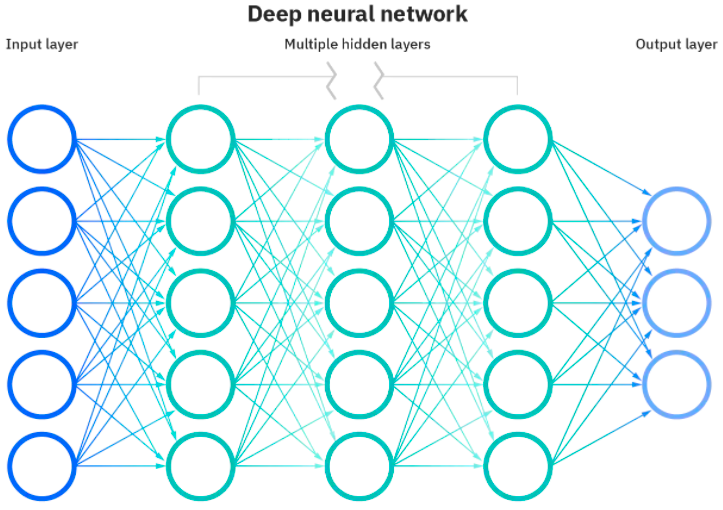
\includegraphics[width=0.7\textwidth]{figures/NN}
	\caption{A figure showing the layers of a Neural Network (see IBM, 2020)}
	\label{firstfig}
\end{figure}\newline
Neural networks depend on training data to learn and improve their accuracy over time. However, once these learning algorithms are polished for accuracy, they become powerful tools in computer science and artificial intelligence, allowing us to classify and cluster data at a high speed. "Tasks in speech recognition or image recognition can take minutes versus hours when compared to the manual identification by human experts" (see IBM, 2020).
\newline\newline
Neural network is good for returns prediction as it can accommodate nonlinear interactions, and no distribution is assumed. However, just like historical simulation they require large data set (which is not always available) for training to perform excellently well.
%%%%%%%%%%%%%%%%%%%%%%%%%%%%%%%%%%%%%%%%%%%%%%%%%%%%%%%%%%%
%%%%%%%%%%%%%%%%%%%%%%%%%%%%%%%%%%%%%%%%%%%%%%%%%%%%%%%%%%%




%%%%%%%%%%%%%%%%%%%%%%%%%%%%%%%%%%%%%%%%%%%%%%%%%%%%%%%%%%%
%%%%%%%%%%%%%%%%%%%%%%%%%%%%%%%%%%%%%%%%%%%%%%%%%%%%%%%%%%%

\section{Mathematics of Neural Network}
The main idea of this section is gotten from the work of Chaoyi Lou, titled Artificial Neural Networks:
their Training Process and Applications.
%%%%%%%%%%%%%%%%%%%%%%%%%%%%%%%%%%%%%%%%%%%%%%%%%%%%%%%%%%%
%%%%%%%%%%%%%%%%%%%%%%%%%%%%%%%%%%%%%%%%%%%%%%%%%%%%%%%%%%%

\subsection{A single Neuron}
\begin{figure}[!h]
	\centering
	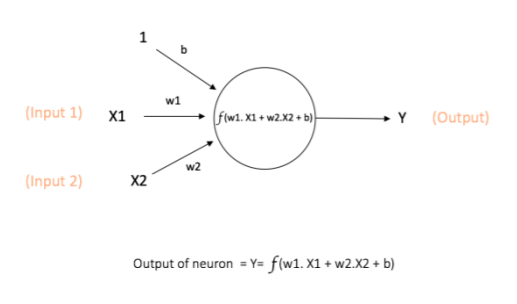
\includegraphics[width=0.7\textwidth]{figures/neuron}
	\caption{A single neuron of neural networks}
	\label{secondfig}
\end{figure}

\autoref{secondfig} shows a network with one layer containing a single neuron. This neuron receives input from the prior input layer, performs computations, and gives output. $x_1$ and $x_2$ are inputs with weights $w_1$ and $w_2$ respectively. The neuron applies a function $f$ to the dot-product of these inputs, which is $w_{1}x{1}+w_{2}x_{2}+b$.  Aside these two numerical input values, there is one input value 1 with weight $b$, called the Bias. The main function of bias is to represent unknown parameters. The dot-product of all input values and their associated weights is fed into the function $f$ to produce the result $Y$.
This function is known as Activation Function.\newline\newline
Activation functions are needed because many problems take multiple influencing factors into account and yield classifications. When faced with a binary classification problem, where the outcomes are either yes or no, activation functions are required to map the outcomes within this range. If a problem involving probability arises, one would expect the neural network's predictions to fall within the range of [0, 1]. This is what activation functions can do.\newline\newline
Linear and non-linear activation functions are the two types of activation functions. The most significant disadvantage of linear ones is that they cannot learn complex function mappings because they are only one-degree polynomials. As a result, non-linear activation functions are always required to produce results in desirable ranges and deliver them as inputs to the next layer. Few of the generally used non-linear activation functions will be discussed in the next section.
\subsection{Activation Functions}
An activation function takes the previously specified dot-product as an input and makes computation with it. Based on the range of the expected result, we place a certain activation function inside hidden layer neurons. The fact that activation functions should be differentiable is important because we'll use it later to train the neural network using backpropagation optimization.
\newline\newline
Here are few commonly used activation functions:\newline\newline
\textbf{Sigmoid}: This takes a real-valued input and returns a output in the range [0,1]:\newline\newline
$\delta = \frac{1}{1+e^{-x}}$
\begin{figure}[!h]
	\centering
	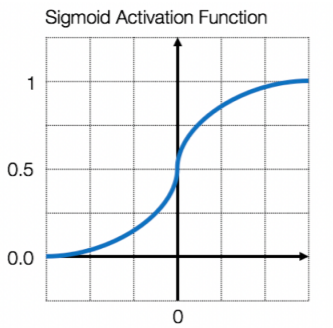
\includegraphics[width=0.4\textwidth]{figures/neuro}
	\caption{Sigmoid() Activation Function}
	\label{thirdfig}
\end{figure}

\autoref{thirdfig} shows an S-shaped curve and the values going
through the Sigmoid function will be squeezed in the range of [0, 1].
As the sigmoid function attains all values between 0 and 1 (with 0 and 1 attained in the limitting cases), the sigmoid function (also called logistic function) is a compatible probability transfer function.
Despite the fact that the Sigmoid function is simple to comprehend and use, it is not widely used due to its vanishing gradient problem. The issue is that the gradient can come so close to zero in some circumstances that it fails to properly adjust the weight. In the worst-case scenario, the neural network's ability to learn will be completely disabled. Second, this function's output is not zero-centered, causing gradient updates to travel in many different directions. Furthermore, the fact that the output is limited to the range [0, 1] makes optimization more difficult.
In order to compensate the deficiencies, tanh() is an alternative option
because it is a stretched version of the Sigmoid function with zero-centered outputs. \newline\newline
\textbf{tanh}: This takes real-valued input and produces the results in the range [-1, 1]:\newline\newline
$\text{tanh(x)}=\frac{sinh(x)}{cosh(x)}=\frac{e^{x}-e^{-x}}{e^{x}+e^{-x}}$

\begin{figure}[!h]
	\centering
	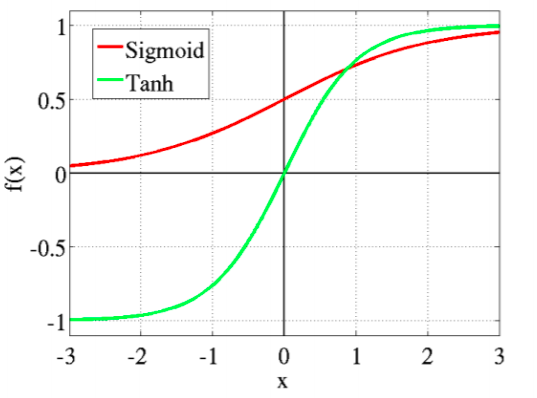
\includegraphics[width=0.4\textwidth]{figures/tanh}
	\caption{tanh() Activation Function}
	\label{fourthfig}
\end{figure}

The benefit of this function is that negative input values will be mapped strongly negative, and extremely small values close to zero will be mapped to values close to zero. As a result, this function is helpful in doing a classification between two classes.
Though in reality, this function is favoured over the Sigmoid function (because of the greater output range), the gradient vanishing problem still occurs. Using a reasonably simple formula, the following ReLU function corrects this problem.\newline\newline

\textbf{ReLU} (Rectified Linear Unit): ReLU is just another name for the positive part of the argument, i.e it takes a real-valued input and replaces the negative values with zero:
\newline\newline
$R(x)= \text{max}(0,x)$
\begin{figure}[!h]
	\centering
	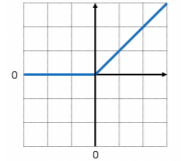
\includegraphics[width=0.4\textwidth]{figures/Relu}
	\caption{ReLU() Activation Function}
	\label{fifthfig}
\end{figure}
\newline\newline As it is a very simple and efficient function that avoids and corrects the gradient vanishing problem, it is employed in practically all convolutional neural networks or deep learning.
The difficulty with this activation function is that after it is activated, all negative values become zeros, which has an impact on the outcomes because negative values are not taken into account.
\newline\newline When we know what qualities of outcomes we want to observe, we apply different activation functions.
 \section{General Model Building}
 Having discussed the mathematics behind neural network, it is however in important to talk about the neural network architectures and other components
 \subsection{Neural network Architures}
 Neural Networks are complex structures made of artificial neurons that can accommodate several inputs to produce output(s). As stated earlier, a Neural Network consists of an input layer, one or multiple hidden layers and output layer(s). In a dense neural network, all the neurons(contained in each layers) affect each other, and hence, they are all connected. How the input neurons produce a certain output is depends
 on the structure of the neural network. The two main classes of network architectures are discussed below
 \subsubsection{Feed-forward Neural Network} (see Bijelic \& Ouijjane, 2019)
 In feed-forward neural network(FFN), each neuron in a
 particular layer is connected with all neurons in a subsequent layer. The information
 flow in the network is of feedforward type (i.e the connections
 can never skip a layer, or form any loops backwards).\newline\newline\newline\newline\newline\newline
 \begin{figure}
 	\centering
 	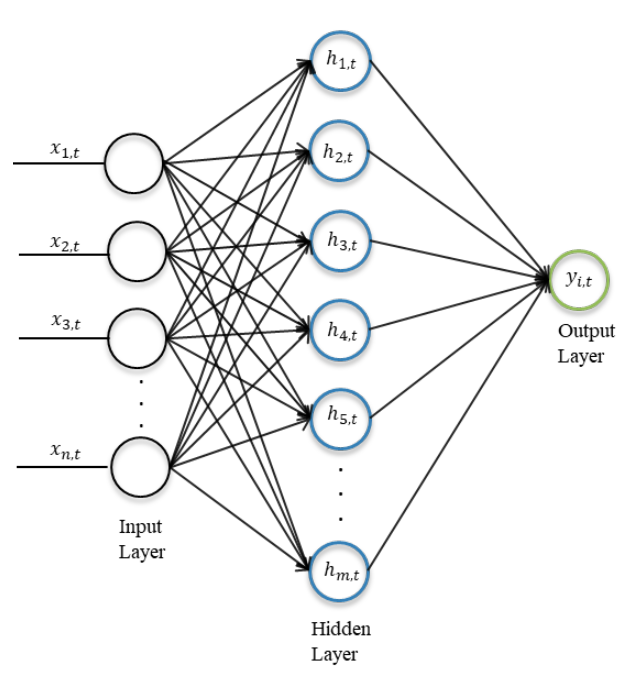
\includegraphics[width=0.4\textwidth]{figures/FFN}
 	\caption{A fully connected FFN with a single hidden layer (see Bijelic \& Ouijjane, 2019)}
 	
 	\label{sixthfig}
 \end{figure}
\newline
 As shown in the above figure, the values of the input are transported to the hidden layer through connections, each being characterised by certain weight coefficient, $W_{i,k}$. The degree of connection between the input node and a hidden node is reflected by these weight coefficients. Defining [$x_{1,t};x_{2,t};...;x_{n,t}$] as the vector of the input signals and [$h_{1,t};h_{2,t};...;h_{m,t}$], the propagation of the input nodes to one hidden node can
 mathematically be described by: \newline
 \begin{center}


 $h_{k,t} =\sum_{i=1}^{n} W_{i,k} \cdot x_{i,t}$ for $k = 1,2,...,m$
  \end{center}
An undesirable property of the formula is its linear representation,
which, if applied, would suggest that the output prediction would be a linear function, which is not always the case. In order to deal with this, a non-linear activation function, $\Phi(\cdot)$ is applied to the weighted sum of
inputs into a hidden node. This activation function, which in the majority of
applications takes the form of a sigmoid function or a ReLu function, makes the neural network a universal approximator i.e neural networks have the capability of approximating
any measurable function to any desired degree
of accuracy, in a very specific and satisfying
sense (see Hornik et al (1989) for details). However, before applying
the activation function, a bias vector [$b_{1};b_{2};...;b_{m}$] is added, which essentially
indicates whether a neuron tends to be active or inactive in the prediction process. The
propagation from the input layer to the hidden layer in a feed-forward neural
network may now be reformulated to:
 \begin{center}
	$h_{k,t} =\Phi(b_{k,0} +\sum_{i=1}^{n} W_{i,k} \cdot x_{i,t}$) for $k = 1,2,...,m$
\end{center}
The feedforward neural network has the major disadvantage that it cannot model temporal dependencies in the data. However, this shortcoming of not being able to account for correlations between inputs is overcome in the recurrent neural network, which is able to selectively feed forward information over sequences of elements by generating cycles in the network.
\subsubsection{Recurrent Neural Network} (see Bijelic \& Ouijjane, 2019)
Recurrent Neural Networks
(RNN) can handle sequential data due to the capability of each neuron to
maintain information about previous inputs, contrary feedforward neural networks. This implies that the prediction a recurrent
neural network node made at previous time step $t-1$ affects the prediction it will make one
moment later, at time step $t$. RNN nodes can be thought of as having memory as it takes inputs not only the current signal, but also
what has been perceived previously in time.\newline\newline
RNNs contain feedback loops from the so-called hidden states, and this allows preservation of information from one node to another while reading in inputs. At each time step in the data series, the feedback loop mechanism occurs, which causes each hidden state to contain traces not only of the respective hidden state before it, but also of all those preceding it, for as long as the memory of the network lasts.\newline

\begin{figure}
	\centering
	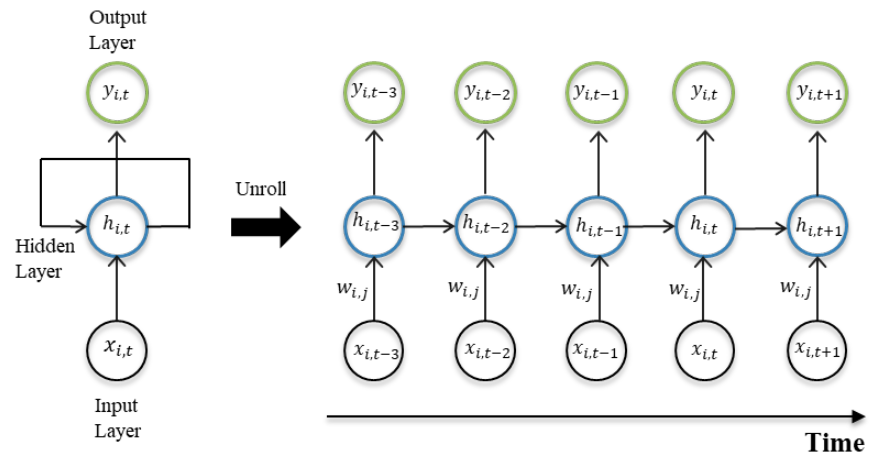
\includegraphics[width=0.4\textwidth]{figures/RNN}
	\caption{Representation of an unrolled plain vanilla recurrent neural network. (see Bijelic \& Ouijjane, 2019)}
	
	\label{seventhfig}
\end{figure}

The unrolled RNN shows how the network enables the hidden neurons to see their
own previous output, so that their subsequent behavior can be shaped by their responses in the past (Tenti, 1996). In addition, utilization of a RNN is particularly desired when there are
time dependencies in the data series, this is evident when we introduce time-lagged model components.
using the initial notation, and suppose that the hidden states are the ones looped
back, the output from a hidden node in the RNN model relies not only on the input values at
time $t$, but also on its own lagged values at order $p$ as represented below:

\begin{center}
	$h_{k,t} =\Phi(b_{k,0} + \sum_{i=1}^{n} W_{i,k} \cdot x_{i,t}) + \sum_{k=1}^{m} \gamma_{k} \cdot h_{k,t-p}$for $k = 1,2,...,m$
\end{center}

where $h_{k,t-p}$ represents the lagged hidden state values at order $p$, and $\gamma_{k}$ a coefficient. Another outstanding feature of recurrent networks is that recurrent neural networks share the same weight parameter within each layer of the network, unlike feedforward networks that have different weights across each node. Through the processes of backpropagation and gradient descent these weights are adjusted to enable reinforcement learning.  Backpropagation through time (BPTT) algorithm is exploited by Recurrent neural networks to determine the gradients, which is a bit different from traditional backpropagation as it is specific to sequence data. In BPTT errors are summed up at each time step whereas feedforward networks do not have to sum errors because it shares no parameter across each layer (see IBM 2020 for details).\newline\newline

In this process, RNNs tend to experience two issues, known as exploding gradients and vanishing gradients. These issues are defined by the gradient size, which is the slope of the loss function along the error curve. If the gradient is too small, the weight parameters will be updated until they become insignificant - i.e. 0, and the algorithm will no longer learn. Gradients explode when they are too large, creating an unstable model. In this case, the model weights will grow too large and will eventually be labelled NaN values. In order to reduce these issues, it is possible to reduce the number of hidden layers within the neural network, thereby reducing its complexity (see IBM 2020).


\subsubsection{Long Short-Term Memory Recurrent Neural Network}
LSTM is a class of recurrent neural networks and its main feature is its purpose-built memory cells, which allows it to capture long range dependencies in the data.\newline\newline
A previous sequence element and the output from the network function serve as input for the next sequence element in the network function. As such, the LSTM can be compared to a HMM (Hidden Markov Model), in which there is a hidden state which conditions the output distribution. Furthermore, LSTM hidden state not only depends on its previous states but also reflects long-term sequence dependence since it is recurrent. In particular, the receptive field size of an LSTM (i.e. the size of the input region that generates the feature) is unbounded architecture-wise, unlike simple feed forward networks and CNNs (see Arimond et al, 2020). \newline\newline Due to the attractiveness of the LSTM, it will be used in this work to forecast volatility of returns of stock markets. \newline\newline

\section{The LSTM Architecture}
Our LSTM has a single hidden layer,  with 'tanh' as the activation function. The following are the hyper parameter (all but MSE has to be determined before you can actually start training, validating and testing your LSTM net) used in within the LSTM neural network:
\begin{itemize}

\item[$\bullet$]   
To determine the best weights of the neural network, Adam (Adaptive Moment Estimation) is the chosen optimizer in our LSTM model. "Some of its advantages are that the sizes of parameter updates are invariant to
rescaling of the gradient, its stepsizes are approximately bounded by the stepsize hyperparameter, stationary objective is not required, it works with sparse gradients, and it naturally performs a
form of step size annealing (see Kingma and Ba, 2015).
\item[$\bullet$] The batch size is the number of inputs that will be propagated in the
LSTM neural network during the training process. In our LSTM model 128 is the chosen batch size, and this means that the inputs are
fed in the network in batches, each containing 128 inputs. After
the propagation of a batch, the network is trained before receiving another
batch of 128 inputs. This operation continues until all inputs are propagated.
\item[$\bullet$] The look ahead is the amount of time steps, i.e. the lagged
inputs the RNN should use to forecast the desired outputs. For all trials, the look back is set to 90 lagged inputs, which
corresponds to about 3-month period in the data sample.
\item[$\bullet$] The dropout function is a regularization method used to prevent overfitting by
allowing the LSTM neural network to drop a random set of neurons while
training the network. Ignoring several neurons for each iteration during the
training process is necessary, because if the network is fully connected,
neurons will become interdependent, leading to overfitting of the training data. For example, if the dropout function is set to 0.25, this means that 25\% of the existing
neurons within the network will be ignored during the training process.
\item[$\bullet$] The number of epochs can also influence the accuracy of a neural network. It
refers to the number of times all the training and validation datasets are
propagated through the LSTM neural network. The standard procedure is to
increase the number of epochs until the chosen metric – in this case the MSE
– decreases for the validation set, while it continues to increase for the training
set, i.e. when the training set shows signs of overfitting.
\item[$\bullet$] The Mean Square Error (MSE): This is the average squared difference between the estimated values and the actual value.
\end{itemize}

\begin{center}
	$L_{MSE} = 1/N\sum_{k=1}^{N} ({\hat{y}}_{k}-y_k)^2$
\end{center}
It is also chosen as the loss function (between the predicted outputs and the actual outputs) and the performance measure(to assess the model fit while
training and validating the network) of the
LSTM neural network
\end{itemize}

The number of neurons, dropout function, and epochs are changed in each LSTM models to choose the one that performs best. That is, the LSTM with the lowest MSE value. This will be discussed in details in the next chapter.


%%%%%%%%%%%%%%%%%%%%%%%%%%%%%%%%%%%%%%%%%%%%%%%%%%%%%%%%%%%
%%%%%%%%%%%%%%%%%%%%%%%%%%%%%%%%%%%%%%%%%%%%%%%%%%%%%%%%%%%
%%%%%%%%%%%%%%%%%%%%%%%%%%%%%%%%%%%%%%%%%%%%%%%%%%%%%%%%%%%
\chapter{Numerical comparisons}
For the empirical study, the day-ahead forecasting of the 1\% and 5\% VAR for daily log-returns(natural log of the new value divided by the initial value) of the following stock markets: NIKKEI 225, FTSE 100 and S\&P 500 is considered. The data is downloaded from DataStream. Each series (NIKKEI 225, FTSE 100 and S\&P 500) consist of 8477 daily price indices (measure of how prices change over a period of time), the start date and end date are 04/01/1988 and 30/06/2020 respectively. Upon calculating the log-returns, which is given as 

\begin{center}
	$R_{log} = ln(\frac{R_f}{R_i})$, where ${R_f}$ and ${R_i}$ are current return and initial return respectively
\end{center}
the data in the first row of the series vanishes leaving us with 8476 daily log-returns and 05/01/1988 as starting date. Basically, this means we use 8476 daily log-returns for our VaR estimations. This longer sample is desirable for our models, most especially the historical simulation and neural network as they work best with large data. Moreover, data contains periods of low and high volatilities, which mitigates the probability of the historical simulation being bias (underestimation or overestimation) in the return estimation.\newline

\begin{figure}[!h]
	\centering
	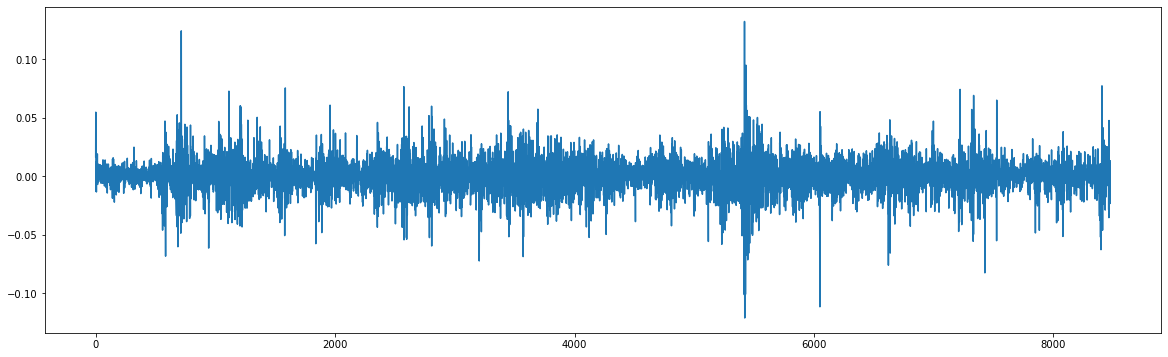
\includegraphics[width=0.8\textwidth]{figures/logNikkei}
	\caption{The series of log-returns of Nikkei 225}
	\label{logNikkei}
\end{figure}

\begin{figure}[!h]
	\centering
	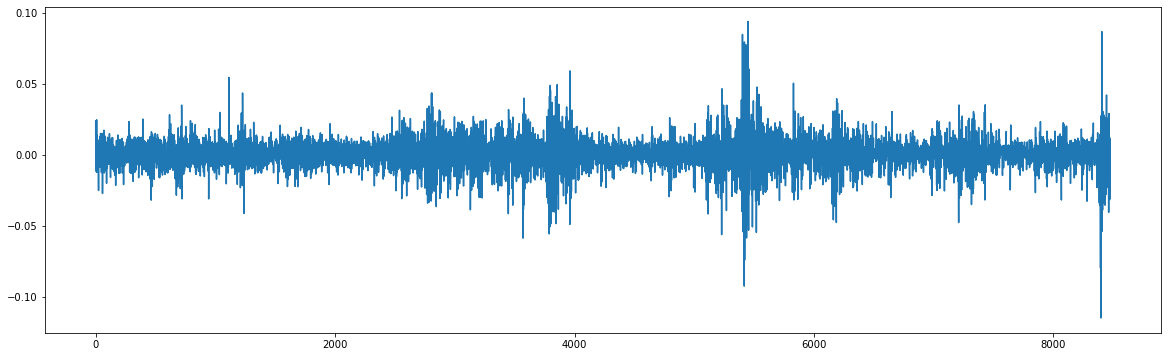
\includegraphics[width=0.8\textwidth]{figures/logFTSE}
	\caption{The series of log-returns of FTSE 100}
	\label{logFTSE}
\end{figure}


\begin{figure}[!h]
	\centering
	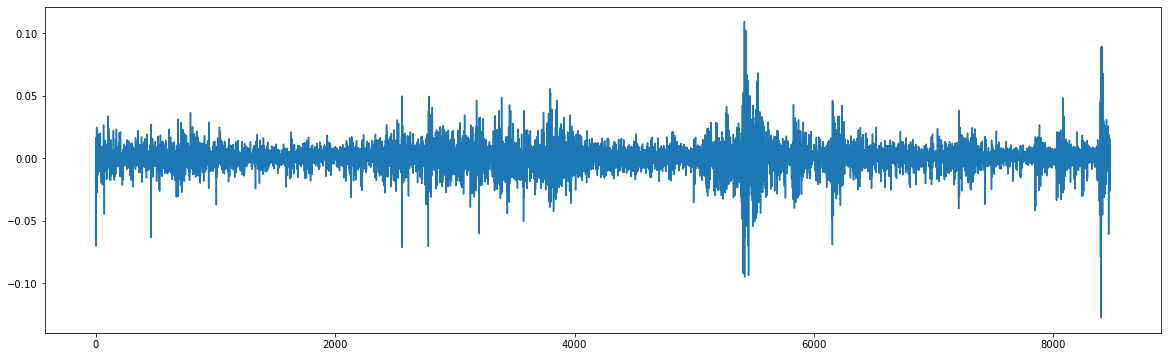
\includegraphics[width=0.8\textwidth]{figures/logS&P500}
	\caption{The series of log-returns of S\&P 500}
	\label{logSandP 500}
\end{figure}

\section{Partitioning the Dataset}
\subsection{LSTM Neural Network Model}

Generally, data is divided into two main parts in neural network models: training set and test set. However, an additional intermediate set called validation set (sometimes modelled as part of training), is sometimes employed in order to avoid overfitting. The training and validation data can be jointly referred to as In-sample data, while the test data is sometimes referred to as Out-of-sample data. In most literatures, the common choice for training set between 70\% to 90\% of the original dataset, and 10\% to 20\% of the training are used as validation dataset. The rest are, of course the testing dataset. \newline\newline

In this study, the first 7000 daily log-returns of each series (each series contains 8476 daily log-returns) are used as training dataset, which is around 83\% of each of the series. The last 700 (10\%) values (daily log-returns) of the training dataset are used for validation. The remaining 1476 daily log-returns are used for testing. However, the first 90 values in our test dataset vanishes due to use of lookahead (timesteps) of 90 days. Apparently, our resultant forecasts (out-of-sample) are 1386 daily log-returns. The dates for the data split are reported in the table below.
%\makeatletter
%\setlength\@fptop{0\p@}
%\makeatother
\newline\newline
\begin{table}[!h]
	\centering
	\begin{tabular}{l|cl}
		\hline \hline
		In-sample
		& out-of-sample\\ \hline
		Training set: 05/01/1988 – 27/02/2012
		& Test set
		: 10/03/2015 – 30/06/2020
	 \\
		Validation set: 28/02/2012– 03/11/2014
		\\
		\hline \hline
	\end{tabular}
	\caption{Data splits}
	%\vspace{128in}
	\label{firsttab}
\end{table}

An important pre-processing step is input normalization, as it is considered good practice for neural network training, data scaling helps neural networks train and converge faster. We use the z-score (StandardScaler): 

\begin{center}
	$X_{new} = \frac{X_{i}-\mu}{\sigma}$
\end{center}

where $X_{new}$ is the standardized data point, $X_{i}$ is the initial data point, $\mu$ is the sample mean and $\sigma$ is the sample standard deviation.


\subsection{Historical simulation and GARCH(1,1) Volatility model}
For congruency with the LSTM model (in regards to number of predictions), we use a rolling window of 7090 for Historical simulation and GARCH(1,1) Volatility model, which stands as our in-sample data and we have 1386 out-of-sample data (predictions).

\subsection{Trial Results of the LSTM Neural Network}

As discussed in the previous chapter, the performance of our LSTM model is based on MSE. In this paper, we follow a best-out-of-5 approach, that means for each stock market, we train our model five times with different values of the hyperparameters and the best one (in each of the model training for the three stock market) is selected for VAR estimation. Tanh is the activation function in all models.\newline
\textbf{NIKKEI}\newline
The training and validation loss continues to decrease as the number of epochs increases until 200 epochs,
after which the model starts to overfit. This was made evident as a result of a slow and steady rise in the
validation loss after 200 epochs, while the training loss keeps reducing.
It was also observed that the most effective size of the LSTM network is 350, and the higher the intensity
of regularization applied, the better the model was able to perform.\newline

\begin{center}
	\begin{tabular}{||c c c c c||} 
		\hline
		Trials & Epochs & Dropout & Hidden Neurons & Validation result\\ [0.5ex] 
		\hline\hline
		1 & 500 & 0.5 & 256 & 0.00036662753 \\ 
		\hline
		2 & 300 & 0.75 & 256 & 0.0001696553 \\
		\hline
		3 & 300 & 0.75 & 350 & 0.00017357965 \\
		\hline
		4 & 200 & 0.5 & 256 & 0.0002184841 \\
		\hline
		5 & 200 & 0.75 & 350 & 0.00016831204\\ [1ex] 
		\hline
	\end{tabular}
\end{center}

In the first trial, the model is trained for 500 epochs, which is more than the desired 200 epochs. The intensity of
regularization is also low at 0.5, the LSTM network size is also low. As a result of the high number of
epochs and low regularization effect, it suffers from the highest variance and produced the worst result.\newline
\begin{figure}[!h]
	\centering
	\includegraphics[width=0.8\textwidth]{figures/Nik1}
	\caption{Training and Validation loss functions under Trial 1 (Nikkei 225))}
	\label{Nik1}
\end{figure}


 The second gives the second best result,as it is trained for more than 200 epochs, and
also the LSTM network at 256 fell short of 350. As a result of this, the model suffers from a higher bias as
compared to the last trial, because the model is not able to learn well as a result of the inadequate LSTM network.\newline\newline\newline\newline\newline\newline\newline\newline\newline\newline\newline
\begin{figure}[!h]
	\centering
	\includegraphics[width=0.8\textwidth]{figures/Nik2}
	\caption{Training and Validation loss functions under Trial 2 (Nikkei 225))}
	\label{Nik2}
\end{figure}

Trial 3 is the third in line, the model is trained for 300 epochs which is longer than the required 200 epochs,
this made the model to suffer from high variance. Since the LSTM is large although the right size, an increase
above the required number of epochs will lead the model to start to overfit rapidly, that was why this trial
performed worse than the second trial.\newline\newline
\begin{figure}[!h]
	\centering
	\includegraphics[width=0.8\textwidth]{figures/Nik3}
	\caption{Training and Validation loss functions under Trial 3 (Nikkei 225))}
	\label{Nik3}
\end{figure}


Trained with the desired 200 epochs, with a low dropout of 0.5, and a low LSTM size of 256. The forth trial
has the lower regularization effect of using a dropout of 0.5 and an insuffcient LSTM
network made the model suffer from higher bias.\newline\newline\newline
\begin{figure}[!h]
	\centering
	\includegraphics[width=0.8\textwidth]{figures/Nik4}
	\caption{Training and Validation loss functions under Trial 4 (Nikkei 225))}
	\label{Nik4}
\end{figure}

The best performed trial is the fifth trial. As a result of the 200 epochs the model trained for being within the range
of avoiding high variance (overfitting) and high bias (underfitting). The dropout regularization intensity is also high enough at 0.75,
and the size of the Long Short Term Memory (LSTM) network at 350 is large enough.\newline
\begin{figure}[!h]
	\centering
	\includegraphics[width=0.8\textwidth]{figures/Nik5}
	\caption{Training and Validation loss functions under Trial 5 (Nikkei 225))}
	\label{Nik5}
\end{figure}
\newline\textbf{FTSE 100}\newline

A decrease in the training and validation loss continues to occur as the number of epochs increases until 205
epochs, after which the model starts to overfit. This is made evident as a result of a slow and steady rise
in the validation loss after 205 epochs, while the training loss keeps reducing.
It was also observed that the most effective size of the LSTM network is 350, and the higher the intensity
of regularization applied, the better the model was able to perform.
\begin{center}
	\begin{tabular}{||c c c c c||} 
		\hline
		Trials & Epochs & Dropout & Hidden Neurons & Validation result\\ [0.5ex] 
		\hline\hline
		1 & 500 & 0.5 & 250 & 0.00013862312 \\ 
		\hline
		2 & 300 & 0.75 & 250 & 0.00012870964 \\
		\hline
		3 & 300 & 0.75 & 350 & 0.000117358715 \\
		\hline
		4 & 200 & 0.5 & 250 & 0.00012332022 \\
		\hline
		5 & 200 & 0.75 & 350 & 0.00011699893\\ [1ex] 
		\hline
	\end{tabular}
\end{center}

The last trial produced the best result, as a result of the 200 epochs used in the training, being within the range
of avoiding high variance and high bias. The dropout regularization intensity is also high enough at 0.75,
and the size of the Long Short Term Memory (LSTM) network at 350 is large enough.
\begin{figure}[!h]
	\centering
	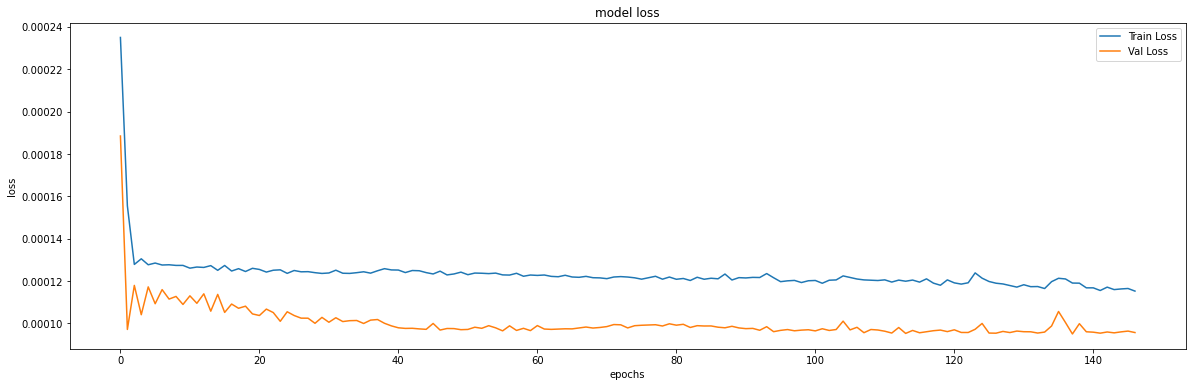
\includegraphics[width=0.8\textwidth]{figures/FTSE5}
	\caption{Training and Validation loss functions under Trial 5 (FTSE 100))}
	\label{FTSE5}
\end{figure}
\newline The third attempt has the second lowest MSE, it fell short because it is trained with more than 200 epochs. As a
result of this, the model suffers from a higher variance as compared to trial 5.\newline\newline\newline\newline\newline\newline\newline\newline\newline\newline\newline\newline
\begin{figure}[!h]
	\centering
	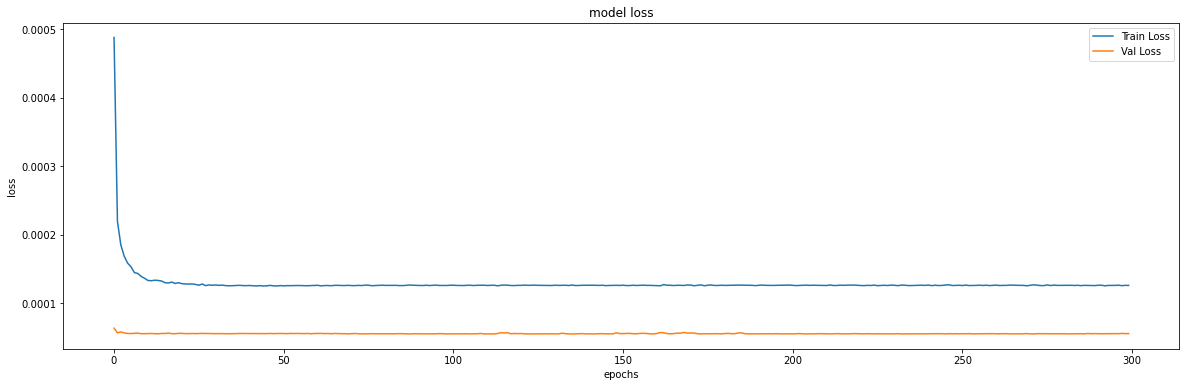
\includegraphics[width=0.8\textwidth]{figures/FTSE3}
	\caption{Training and Validation loss functions under Trial 3 (FTSE 100))}
	\label{FTSE3}
\end{figure}
\newline Although, the forth trial is trained with the required 200 epochs but fall short, as a result of the low dropout of 0.5 and inadequate
LSTM network size. The low regularization intensity had the greatest effect, leading to high variance.\newline
\begin{figure}[!h]
	\centering
	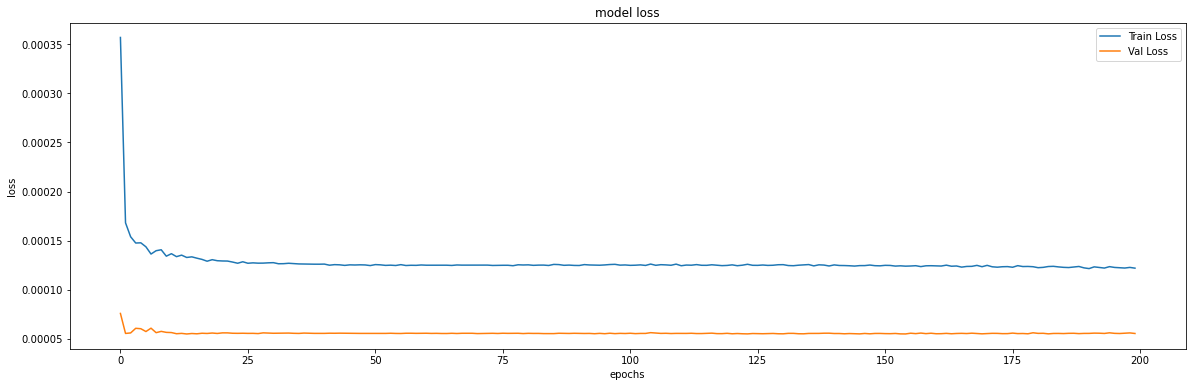
\includegraphics[width=0.8\textwidth]{figures/FTSE4}
	\caption{Training and Validation loss functions under Trial 4 (FTSE 100))}
	\label{FTSE4}
\end{figure}
\newline The second trial is overtrained for 300 epochs, the dropout at 0.5 is low, and the LSTM network at 250, are what
led to a less impressive result compared to trial 5,3, and 4 \newline\newline\newline

\begin{figure}[!h]
	\centering
	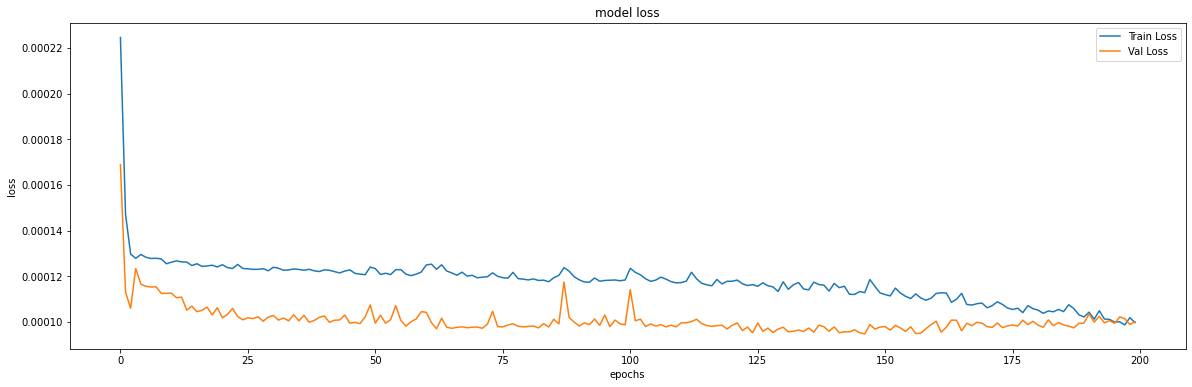
\includegraphics[width=0.8\textwidth]{figures/FTSE2}
	\caption{Training and Validation loss functions under Trial 2 (FTSE 100))}
	\label{FTSE2}
\end{figure}

 Suffers the same set back as the second trial, the first trial is trained with an even larger number of epochs at 500. This made it
perform the worst in comparison with the rest of the trails.\newline\newline\newline
\begin{figure}[!h]
	\centering
	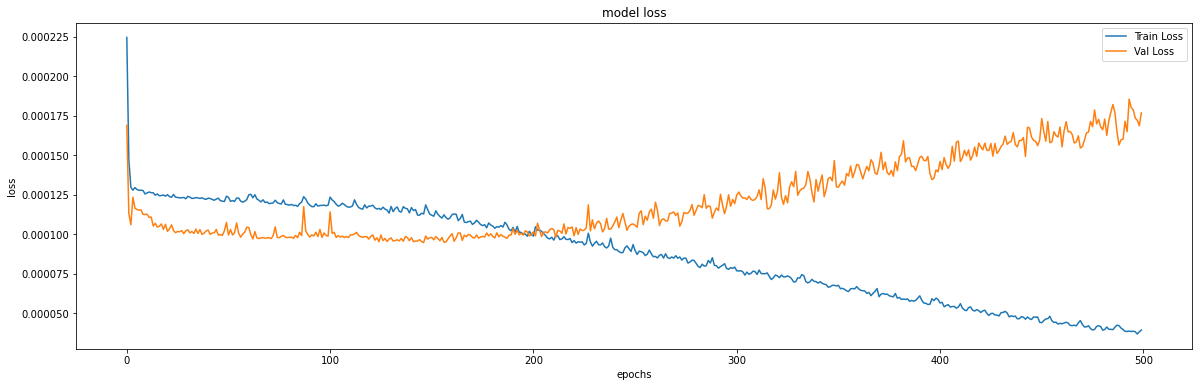
\includegraphics[width=0.8\textwidth]{figures/FTSE1}
	\caption{Training and Validation loss functions under Trial 1 (FTSE 100))}
	\label{FTSE1}
\end{figure}
 
 
 \textbf{S\&P500}\newline\newline
A decrease in the training and validation loss continues to occur as the number of epochs increases until 270
epochs, after which the model starts to overfit. This was made evident as a result of a slow and steady rise
in the validation loss after 270 epochs, while the training loss keeps reducing.

\begin{center}
	\begin{tabular}{||c c c c c||} 
		\hline
		Trials & Epochs & Dropout & Hidden Neurons & Validation result\\ [0.5ex] 
		\hline\hline
		1 & 500 & 0.5 & 250 & 0.00020557812 \\ 
		\hline
		2 & 300 & 0.75 & 250 & 0.00017026176 \\
		\hline
		3 & 300 & 0.75 & 350 & 0.00013683487 \\
		\hline
		4 & 270 & 0.5 & 256 & 0.00015936441 \\
		\hline
		5 & 270 & 0.8 & 356 & 0.00013847416 \\ [1ex] 
		\hline
	\end{tabular}
\end{center}



With the largest number of epochs of 500. The first trial suffers from severe overfitting, and made it perform the worst compared to the rest of the trials.\newline
\begin{figure}[!h]
	\centering
	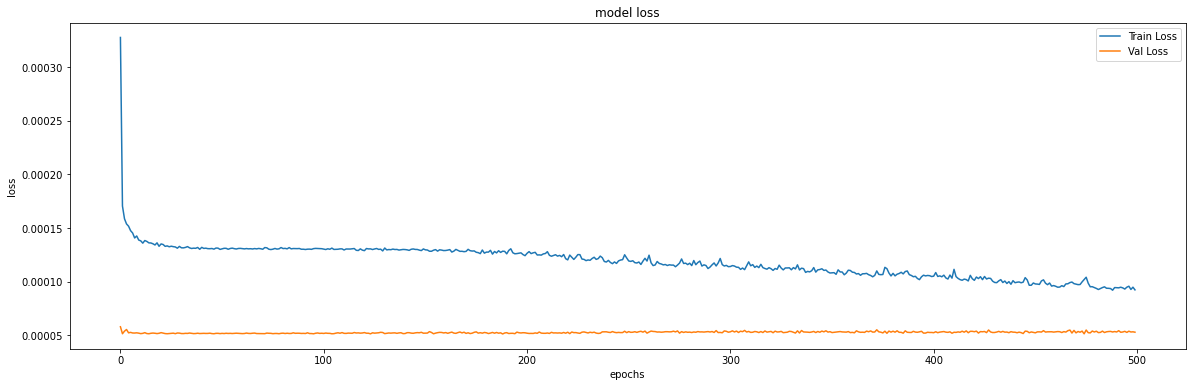
\includegraphics[width=0.8\textwidth]{figures/sanp1}
	\caption{Training and Validation loss functions under Trial 1 (S\&P 500)}
	\label{sanp1}
\end{figure}
\newline The second trial is modelled with 300 epochs, the dropout at 0.5 is low, and the LSTM network at 250 neurons, are what
led to a less impressive result compared to the subsequent trials. \newline\newline\newline\newline\newline\newline\newline\newline\newline\newline\newline
\begin{figure}[!h]
	\centering
	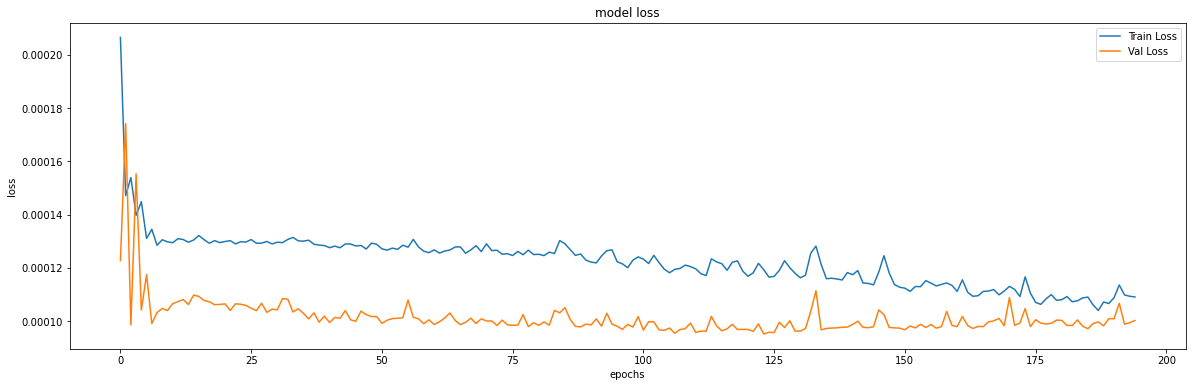
\includegraphics[width=0.8\textwidth]{figures/sanp2}
	\caption{Training and Validation loss functions under Trial 2 (S\&P 500)}
	\label{sanp2}
\end{figure}
\newline The third attempt has the same number of epochs as second trial, produced the least MSE value, but still suffers from much overfitting despite increasing the dropout and the number of neurons.\newline
\begin{figure}[!h]
	\centering
	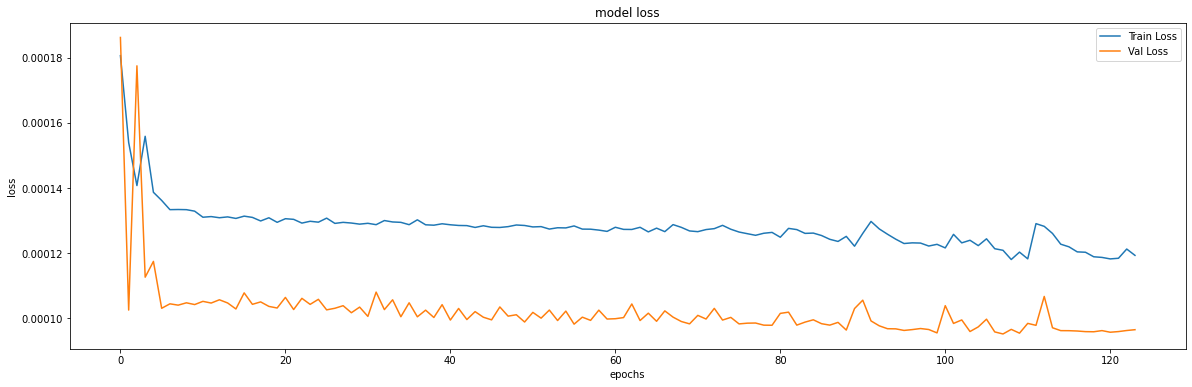
\includegraphics[width=0.8\textwidth]{figures/sanp3}
	\caption{Training and Validation loss functions under Trial 3 (S\&P 500)}
	\label{sanp3}
\end{figure}

The penultimate trial is trained with the sufficient 270 epochs, but as a result of the low dropout of 0.5 and inadequate LSTM
network size. The low regularization intensity has the greatest effect, leading to high variance.\newline
\begin{figure}[!h]
	\centering
	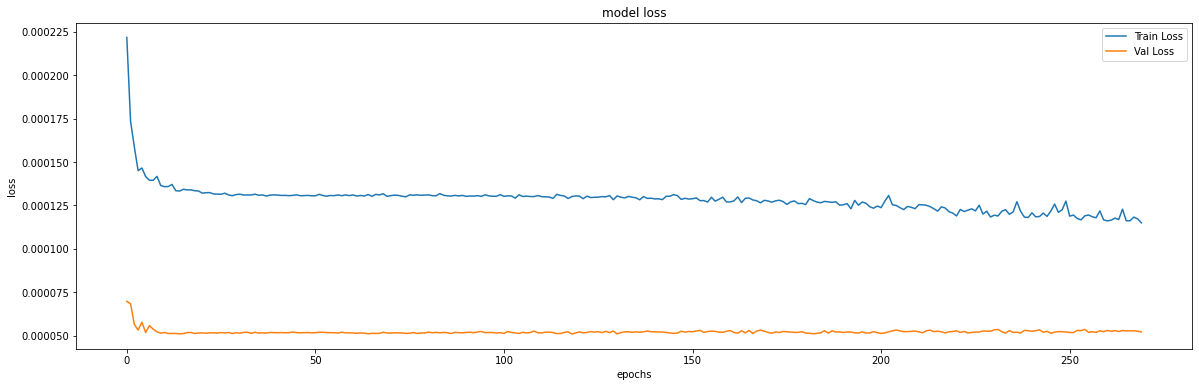
\includegraphics[width=0.8\textwidth]{figures/sanp4}
	\caption{Training and Validation loss functions under Trial 4 (S\&P 500)}
	\label{sanp4}
\end{figure}
\newline The final trial is trained with 270 epochs and the increased number of hidden neurons and dropout made it outperform the fourth trial and this is considered the best model.
\begin{figure}[!h]
	\centering
	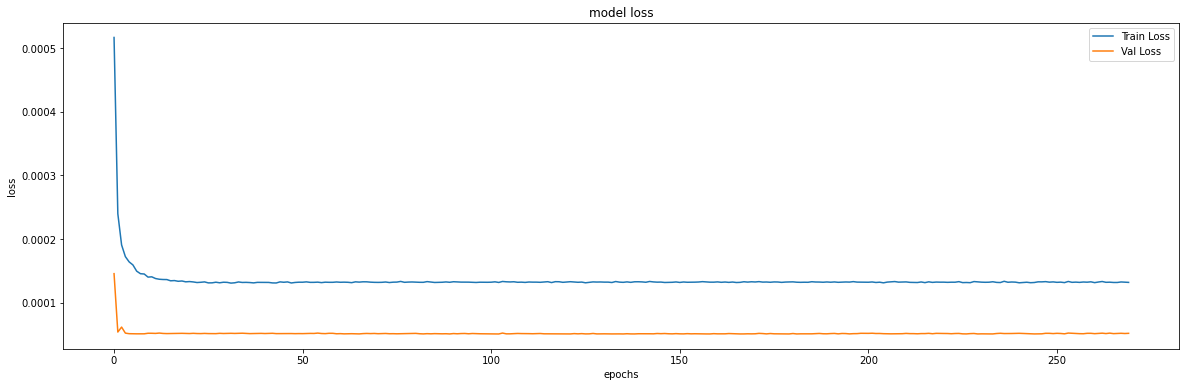
\includegraphics[width=0.8\textwidth]{figures/sanp5}
	\caption{Training and Validation loss functions under Trial 5 (S\&P 500)}
	\label{sanp5}
\end{figure}\newline\newline\newline\newline\newline

\section{VAR Estimation}
In this section, we discuss the estimation of our value at risk.
\subsection{Historical Simulation}
As a nonparametric method, we use historical simulation with rolling window of 7090 observations to estimate the value at risk for the next 1386 days.



\subsection{GARCH (1,1) model}

For our VaR estimation, we use the conditional variance given by GARCH(1,1) model. We assume the random error to have a student’s t-distribution. Our Value at Risk is given by:
\begin{center}
$\text{VaR}_{t+1|t}$ = $\mu_{t+1|t} + \sigma_{t+1|t} * q_{\alpha}$
\end{center}
where $\mu$ is the conditional mean, $\sigma$ is the conditional volatility, and $q_{\alpha}$ is the $\alpha$ quantile of the standardized residuals.

\subsection{The LSTM model}
We determine our value at risk by calculating the 0.05 quantile (95\% Var) and 0.01 (99\% Var) of our predicted values. Our LSTM model equation is assumed to be of the form:
\begin{center}
	$y_1= tanh(\sum_{i=1}^{i=90}W_{i}u_{i}+\beta)+\varepsilon_t$
\end{center} 

where $u_{i}$ are the inputs(initial timesteps), $W_i$ are the weights, $\beta$ is the bias and $\varepsilon_t$ is the error term which has a standard normal distribution, tanh is the activation function. As the output from the network function serves as input for the next sequence element in the network function, the general equation would be of the form:

\begin{center}
	$y_n= tanh(\sum_{i=1}^{i=90}W_{i}u_{i}+\sum_{i=1}^{n-1}y_{i}K_{i}+\beta)+\varepsilon_t$
\end{center} 
where $K_i$ are weights, $y_i$ are initial outputs.

\section{VAR Backtesting}
%\subsection{Binomial Test}
One easy way to test the efficiency of a VaR model is to count the number of violation (number of days when portfolio returns are less than VaR model estimates). A VaR model performs overestimation of risk if the number of exceptions is less than the selected confidence level, and underestimation if there are too much violation. It is nearly impossible to have the exact amount of violation specified by the confidence level.\newline\newline

Suppose we use a 99\% confidence for our VaR model, we have $K$ as the number of violations and N observations. The ratio $k$/$N$ gives the failure rate. Our null hypothesis is that the frequency of tail loss is $p$= 0.01. Assuming that the model is accurate, the observed failure rate $k$/$N$
should act as an unbiased measure of p, and thus converge to 1\% as sample size is
increased. (Jorion, 2007) \newline\newline
It is based on the classic testing framework for a series of successes and failures, also known as Bernoulli tests. Under the null hypothesis, the number of violations(breaches) k follows a binomial probability distribution:
\begin{center}
	$f(k)$ =$N \choose {k}$ $p^{k}(1-p)^{N-k}$ 
\end{center}

By applying the central limit theorem, we can approximate the binomial distribution by the normal distribution when T is large
\begin{center}
	$z$ =$\frac{k-pN}{\sqrt{p(1-p)T}}\sim N(0,1)$ 
\end{center}
(see Jorion, 2007).

\subsection{Kupiec POF-Test}
Kupiec POF-test (proportion of failures) is based on failure rate and was propose by Kupiec (1995). Under null
hypothesis that the model is correct, the number of violations follows the
binomial distribution. According to Kupiec
(1995), the POF-test is best conducted as a likelihood-ratio (LR) test. The test
statistic takes the form
\begin{center}
	$LR_{pof}$ =$-2\ln$ $\left(\frac{(1-p)^{N-k}p^k}{[1-(k/N)]^{N-k}(k/N)^k}\right)$
\end{center}
$LR_{pof}$ (when $N$ is large) is asymptotically $\chi^2$ distributed with one degree of freedom under the null hypothesis that our model is correct. Thus our null hypothesis will be rejected if $LR_{pof}$ is greater than the critical value of the $\chi^2$ significant level (see Jorion, 2007). It is common to choose a 95\% confidence level for backtesting and apply this level to different VaR models regardless of the VaR confidence level chosen.


\subsection{Results}
For congruency with the VaR calculated from our LSTM forecasts, we calculate our actual VaR as the average of daily VaRs stimulated in the Garch and historical simulation model, and this actual VaR is used for comparison with our out-of sample data.




\begin{table}[h]
	\caption {VaR results for Nikkei 225}
	\centering\setlength{\extrarowheight}{2pt}
	\centering
	\begin{tabular}{|*{7}{c|}}
		\hline
		\multirowcell{3}{model} & 
		
		\multicolumn{2}{c|}{VaR} & \multicolumn{2}{c|}{No. of VAR breaches} &
		\multicolumn{2}{c|}{kupiec 95\% test} \\
		\cline{2-7}
		&  \makecell{95\%} & \makecell{99\%} & \makecell{95\%} & \makecell{99\%} & \makecell{95\%} & \makecell{99\%} \\
		\hline
		Historical Simulation  & -0.023307  & -0.039578 &   57  & 16  & 2.44  & 0.318 \\ 
		\hline
		Garch(1,1) model &  -0.019251 & -0.031422 & 82   &  29 & 2.32  & 12.71 \\
		\hline
		NN model & 0.75 & 350 &    &   &    &  \\
		\hline
	\end{tabular}
\end{table}


\begin{table}[h]
	\caption {VaR results for FTSE 100}
	\centering\setlength{\extrarowheight}{2pt}
	\centering
	\begin{tabular}{|*{7}{c|}}
		\hline
		\multirowcell{3}{model} & 
		
		\multicolumn{2}{c|}{VaR} & \multicolumn{2}{c|}{No. of VAR breaches} &
		\multicolumn{2}{c|}{kupiec 95\% test} \\
		\cline{2-7}
		&  \makecell{95\%} & \makecell{99\%} & \makecell{95\%} & \makecell{99\%} & \makecell{95\%} & \makecell{99\%} \\
		\hline
		Historical Simulation  & -0.016711 & -0.030739 &   61  & 21  & 1.09  & 3.21 \\ 
		\hline
		Garch(1,1) model & -0.014778  & -0.022997 &  73  &  40 & 0.20  & 33.01 \\
		\hline
		NN model & 0.75 & 350 &    &   &    &  \\
		\hline
	\end{tabular}
\end{table}



\begin{table}[h]
	\caption {VaR results for S\&P 500}
	\centering\setlength{\extrarowheight}{2pt}
	\centering
	\begin{tabular}{|*{7}{c|}}
		\hline
		\multirowcell{3}{model} & 
		
		\multicolumn{2}{c|}{VaR} & \multicolumn{2}{c|}{No. of VAR breaches} &
		\multicolumn{2}{c|}{kupiec 95\% test} \\
		\cline{2-7}
		&  \makecell{95\%} & \makecell{99\%} & \makecell{95\%} & \makecell{99\%} & \makecell{95\%} & \makecell{99\%} \\
		\hline
		Historical Simulation  & -0.017029 & -0.031004 &  70   & 21  &  0.007 & 3.21 \\ 
		\hline
		Garch(1,1) model & -0.014281 & -0.023931 &  91  &  39 & 6.54 & 30.88 \\
		\hline
		NN model & -0.018751 & 0.029418 &   57 & 26  &  2.44  & 8.54 \\
		\hline
	\end{tabular}
\end{table}





%%%%%%%%%%%%%%%%%%%%%%%%%%%%%%%%%%%%%%%%%%%%%%%%%%%%%%%%%%%
%%%%%%%%%%%%%%%%%%%%%%%%%%%%%%%%%%%%%%%%%%%%%%%%%%%%%%%%%%%
%%%%%%%%%%%%%%%%%%%%%%%%%%%%%%%%%%%%%%%%%%%%%%%%%%%%%%%%%%%


%%%%%%%%%%%%%%%%%%%%%%%%%%%%%%%%%%%%%%%%%%%%%%%%%%%%%%%%%%%
%%%%%%%%%%%%%%%%%%%%%%%%%%%%%%%%%%%%%%%%%%%%%%%%%%%%%%%%%%%
%%%%%%%%%%%%%%%%%%%%%%%%%%%%%%%%%%%%%%%%%%%%%%%%%%%%%%%%%%%

\begin{appendix}
		\chapter{}
	
	Graphs of log-return series of each stock market	
	

	%%%%%%%%%%%%%%%%%%%%%%%%%%%%%%%%%%%%%%%%%%%%%%%%%%%%%%%%%%%
	%%%%%%%%%%%%%%%%%%%%%%%%%%%%%%%%%%%%%%%%%%%%%%%%%%%%%%%%%%%

	\chapter{}

	%%%%%%%%%%%%%%%%%%%%%%%%%%%%%%%%%%%%%%%%%%%%%%%%%%%%%%%%%%%
	
In all the graphs below, number of epochs is represented by the
horizontal axis (X-axis), while the loss functions are represented by the vertical axis
(Y-axis).



	
	
	






	%%%%%%%%%%%%%%%%%%%%%%%%%%%%%%%%%%%%%%%%%%%%%%%%%%%%%%%%%%%\\
	%%%%%%%%%%%%%%%%%%%%%%%%%%%%%%%%%%%%%%%%%%%%%%%%%%%%%%%%%%%
	
	\chapter{Another example}
	\label{app_ex2}
	
	%%%%%%%%%%%%%%%%%%%%%%%%%%%%%%%%%%%%%%%%%%%%%%%%%%%%%%%%%%%
	
	\section{More stuff}
	
	Bla bla.
	
\end{appendix}

%%%%%%%%%%%%%%%%%%%%%%%%%%%%%%%%%%%%%%%%%%%%%%%%%%%%%%%%%%%
%%%%%%%%%%%%%%%%%%%%%%%%%%%%%%%%%%%%%%%%%%%%%%%%%%%%%%%%%%%
%%%%%%%%%%%%%%%%%%%%%%%%%%%%%%%%%%%%%%%%%%%%%%%%%%%%%%%%%%%

\bibliographystyle{plain}
\bibliographystyle{abbrvnat}
\bibliography{literature/library}
Acerbi, C. and Tasche, D. On the coherence of expected shortfall, \textit{Journal of Banking and Finance}, Vol. 26, 2002,
pp. 1496-1500.\newline\newline
Jorion, P. Value at Risk: The New Benchmark for Managing Financial Risk, McGraw-Hill, 2007.\newline\newline
Sun, W., Rachev, S., Chen, Y and Fabozzi, F., (2008). Measuring Intra-Day Market
Risk: A Neural Network Approach.\newline\newline
James W. Taylor (2019). Forecasting Value at Risk and Expected Shortfall
Using a Semiparametric Approach Based on the Asymmetric Laplace Distribution, \textit{Journal of
Business \& Economic Statistics}, 37:1, 121-133.\newline\newline
Patton, A.J., Ziegel, J.F., Chen, R. (2019). Dynamic semiparametric models for expected shortfall
(and Value-at-Risk), \textit{Journal of Econometrics}, 211, 388-413.\newline\newline
Arimond A., et al (2020). Neural Networks and Value at Risk. 	arXiv:2005.01686\newline\newline
Nagai M. (2016) Estimation of Extreme Value at Risks Using CAViaR Models, \textit{Graduate School of Economics, Hitotsubashi University}.\newline\newline
Abed, P., Benito, S., (2013). A detailed comparison of value at risk estimates, \textit{Mathematics and Computers in Simulation}, 94, 258–276.\newline\newline
Abed, P., Benito, S., (2009). A Detailed Comparison of Value at Risk in International Stock Exchanges\newline\newline
Graves, A. (2013). Generating sequences with recurrent neural networks. arXiv preprint arXiv:1308.0850.\newline\newline
Abed, P., Benito, S., Lopez, C. A comprehensive review of Value at Risk methodologies, \textit{Spanish Review of Financial Economics} 12(1), 2013. \\\\
Ruilova, J.C., Morettin P. A., (2020). Parsimonious Heterogeneous ARCH Models for High
Frequency Modeling, \textit{Journal of Risk and Financial Management}.\\\\
Yu, P., Yan, X. Stock price prediction based on deep neural networks, \textit{Journal of Neural Computing and Applications} 32(5), 2020.\\\\
Buczyński, Mateusz; Chlebus, Marcin (2018) : Comparison of semiparametric
and benchmark value-at-risk models in several time periods with different volatility
levels, \textit{e-Finanse: Financial Internet Quarterly, ISSN 1734-039X, University of Information
Technology and Management, Rzeszów, Vol. 14, Iss. 2, pp. 67-82,
http://dx.doi.org/10.2478/fiqf-2018-0013}\\\\
Bijelic \& Ouijjane (2019) : Predicting Exchange Rate
Value-at-Risk and Expected Shortfall:
A Neural Network Approach. \textit{Master thesis, School of Economics and Management, Lund University}.\\\\
Kingma, D. and Ba, J. (2015) Adam: A Method for Stochastic Optimization. \textit{Proceedings of the 3rd International Conference on Learning Representations (ICLR 2015)}.\\\\
Teo Li Hui (2006) : Comparison of Value-At-Risk (VAR) Using Delta-Gamma
Approximation with Higher Order Approach. \textit{Master thesis, Department of Mathematics, National University of Singapore}.\\\\
James W. Taylor (2020). Forecast combinations for value at risk and expected shortfall, \textit{International Journal of Forecasting}, 36, 428-441.\\\\
Chaoyi Lou (2019). Artificial Neural Networks:
their Training Process and Applications \textit{Department of Mathematics, Whitman College}.\\\\
IBM (2020). Neural Networks, https://www.ibm.com/cloud/learn/neural-networks\\\\
IBM (2020). Recurrent Neural Networks, https://www.ibm.com/cloud/learn/recurrent-neural-networks\\\\
Brownlee, J., (2016). Time Series Prediction with LSTM Recurrent Neural Networks
in Python with Keras, Deep Learning for time series.\\\\
Locarek-Junge, H. and Prinzler, R. (1999). Using ANN to Estimate VaR, working
paper.\\\\
S. A. Hamid and Z. Iqbal. Using neural networks for forecasting volatility of S\&P 500 Index futures prices \textit{Journal of Business Research 57 (2004) 1116–1125}.\\\\
He, K., Ji, L., Tso, G. K. F., Zhu, B., \& Zou, Y. (2018). Forecasting Exchange Rate Value at Risk using Deep Belief Network Ensemble based Approach. \textit{Procedia Computer Science}, 139, 25-32.
https://doi.org/10.1016/j.procs.2018.10.213.





\listoffigures
\listoftables

%\printindex

%%%%%%%%%%%%%%%%%%%%%%%%%%%%%%%%%%%%%%%%%%%%%%%%%%%%%%%%%%%
%%%%%%%%%%%%%%%%%%%%%%%%%%%%%%%%%%%%%%%%%%%%%%%%%%%%%%%%%%%
%%%%%%%%%%%%%%%%%%%%%%%%%%%%%%%%%%%%%%%%%%%%%%%%%%%%%%%%%%%
\end{document}

%%%%%%%%%%%%%%%%%%%%%%%%%%%%%%%%%%%%%%%%%%%%%%%%%%%%%%%%%%%
